\documentclass{article}

\usepackage[a4paper]{geometry}
\usepackage[ngerman]{babel}
\usepackage[utf8]{inputenc}
\usepackage[T1]{fontenc}
\usepackage{graphicx}
\usepackage{fancyhdr}
\usepackage{xcolor}
\usepackage{float}

\graphicspath{{./images/}}

\pagestyle{fancyplain}
\fancyhf{}
\lhead{\fancyplain{}{Mara Schulke} }
\rhead{\fancyplain{}{\today}}
\cfoot{\fancyplain{}{\thepage}}

\begin{document}

\begin{titlepage}
	\begin{flushleft}
		TH Brandenburg \\
		Online Studiengang IT Sicherheit \\
		Fachbereich Informatik und Medien \\
		Digitaler Selbstschutz \\
		Prof.\ Dr.\ Michael Pilgermann
	\end{flushleft}

	\vfill

	\begin{center}
		\Large{Hausarbeit: Schutz des THB-Webmail-Accounts mit einem 2. Faktor}\\[0.5em]
		\large{Wintersemester 2022}\\[0.25em]
		\large{Abgabetermin \today}
	\end{center}

	\vfill

	\begin{flushright}
		Mara Schulke \\
		Matrikel-Nr. 20215853
	\end{flushright}
\end{titlepage}

\begin{abstract}
	Durch die Implementierung von 2-Faktor-Authentifizierung können bestehende
	Systeme hinsichtlich ihrer Sicherheit stark verbessert werden und neue
	Systeme grundlegend neue Authentifizierungskonzepte implementieren. Die
	Unterstützung der Industrie zeigt sich durch die Implementierung durch große
	Firmen. Durch die Verwendung von ausgereiften
	Bibliotheken für die Generierung und Validierung von
	\textit{One-Time-Passwords} kurz \textit{OTP} sind schnelle und
	zuverlässige Implementierungen des Standards leicht realisierbar.
\end{abstract}

\tableofcontents

\listoffigures

\newpage

\section{Einleitung}

Authentifizierung ist eines der größten Probleme, die durch verteilte Systeme
entstehen. Es gibt zahlreiche Möglichkeiten, die Identität einer Gegenseite
sicherzustellen allerdings weisen viele von ihnen Schwachstellen hinsichtlich
Man-In-The-Middle-Attacken und basieren auf der Annahme, dass das System des
Nutzers nicht kompromittiert wurde. Als eine mögliche Lösung für viele dieser
Probleme hat sich die 2-Faktor-Authentifizierung innerhalb der letzten Jahre zu
einem beliebten Standard entwickelt, der von vielen großen Anbietern wie
Facebook, Amazon, Google, Mozilla, Microsoft etc.\ bereits unterstützt
wird.

\subsection{Welche Probleme löst die Zwei-Faktor-Authentifizierung?}

Die Notwendigkeit für einen solchen Standard hat sich in den letzten Jahren
immer stärker gezeigt, da die klassische Passwort-Authentifizierung (1-Faktor)
durch zunehmende Rechenleistung und effizientere Angriffe immer unsicherer und
unhandlicher für Nutzer wird. Die minimalen Passwortlängen steigen
dementsprechend an und führen zur Wiederverwendung von gleichen Login-Daten für
mehrere Online-Dienste. Bekannte Lösungen sind die Verwendung von sogenannten
Passwort-Managern um lange und zufällige Passwörter für verschiedenste
Online-Dienste zu verwenden, ohne dass sich Nutzer diese merken müssen. Solche
Passwort-Manager sind zwar eine Lösung für die sichere Aufbewahrung von langen
Passwörtern, können aber nicht die grundsätzlich durch
Passwort-Authentifizierung eröffneten Angriffsvektoren wie zum Beispiel
Man-In-The-Middle-Attacken. So bald ein Angreifer in den Besitz des geheimen
Wissens (in diesem Fall das Passwort) gelangt, kann dieser uneingeschränkt und
unbegrenzt oft auf das Zielsystem zugreifen, bis der Nutzer seine Daten
ändert (vorausgesetzt, der Angreifer hat dies noch nicht getan).

Durch den Wechsel von einer reinen Passwort-Authentifizierung auf
Zero-Knowledge-Proof basierte Authentifizierungsmethoden (in diesem Fall
One-Time-Passwords) lassen sich ganze Angriffsvektoren ausschließen,
da ein kompromittierter Server oder eine kompromittierte Verbindung niemals das
gesamte geheime Wissen des Nutzers einem Angreifer zugänglich machen. Das
heißt, dass sich ein Angreifer im Falle einer kompromittierten Verbindung
maximal in die Sitzung des Nutzers einschleichen könnte, allerdings bei der
nächsten Authentifizierung nicht erneut die Identität des Nutzers beweisen
könnte und somit den Zugriff verlieren würde.

Im Falle der Zwei-Faktor-Authentifizierung kennt nicht einmal das System des
Nutzers das Geheimnis um valide One-Time-Passwörter zu generieren, da
dieses auf einem externen Gerät (in der Regel das Smartphone) verwaltet werden
und der Beweis des Besitzes durch die Eingabe des OTP erfolgt. So stellt selbst
ein kompromittiertes Nutzersystem nur eine temporäre Schwachstelle dar, da
immer nur die jeweiligen OTP abgegriffen werden können, aber nie das Geheimnis
zur Generierung dieser.

\section{Einrichtung einer 2-Faktor-Authentifizierung bei Zimbra}

Die Einrichtung einer App zur 2-Faktor-Authentifizierung ist dank des
Einreichtungsassistenten unkompliziert und weitgehend nutzerfreundlich. Die
Einrichtung kann nach erfolgreichem Login unter der Einstellungsseite im Reiter
``Accounts'' vorgenommen werden. (Abb. 1)

\begin{figure}[H]
	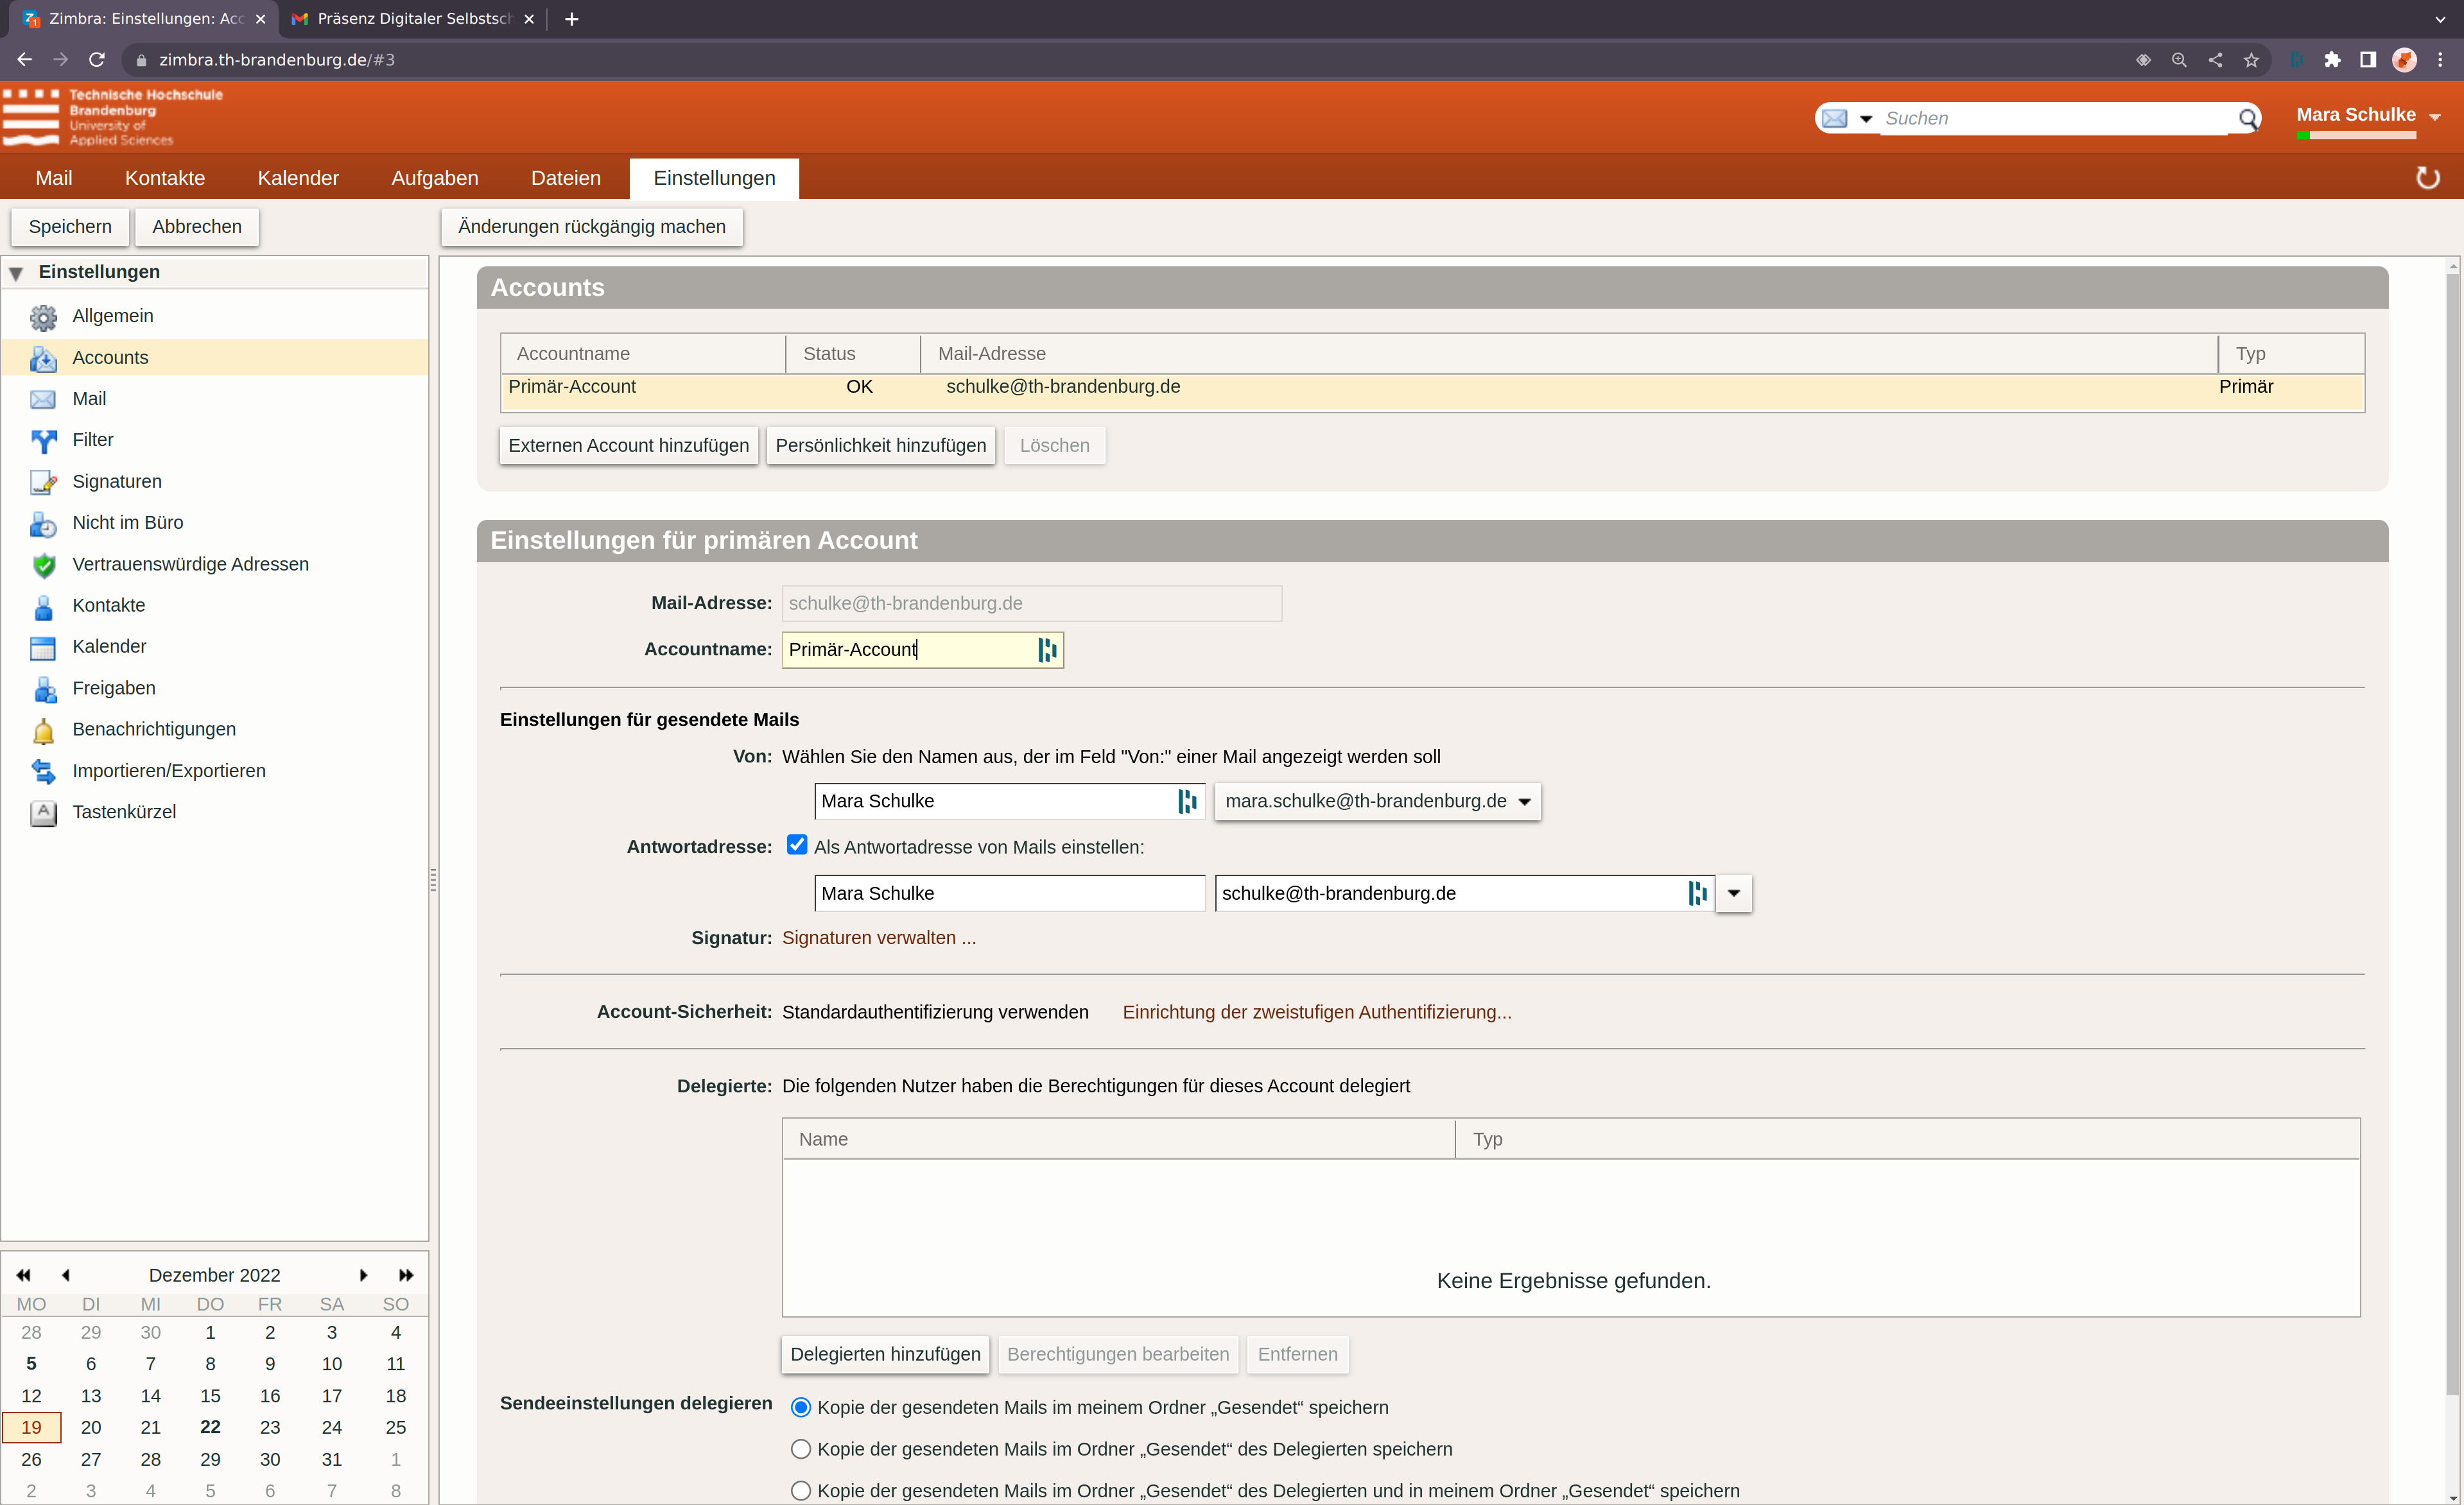
\includegraphics[width=0.75\textwidth]{images/01-einstellung.png}
	\centering
	\caption{Einstelungen Zimbra}
\end{figure}

Zu Beginn der Einrichtung werden wichtige Hinweise zur
2-Faktor-Authentifizierung angezeigt und dem Nutzer wird die Funktionsweise
erklärt. (Abb. 2)

\begin{figure}[H]
	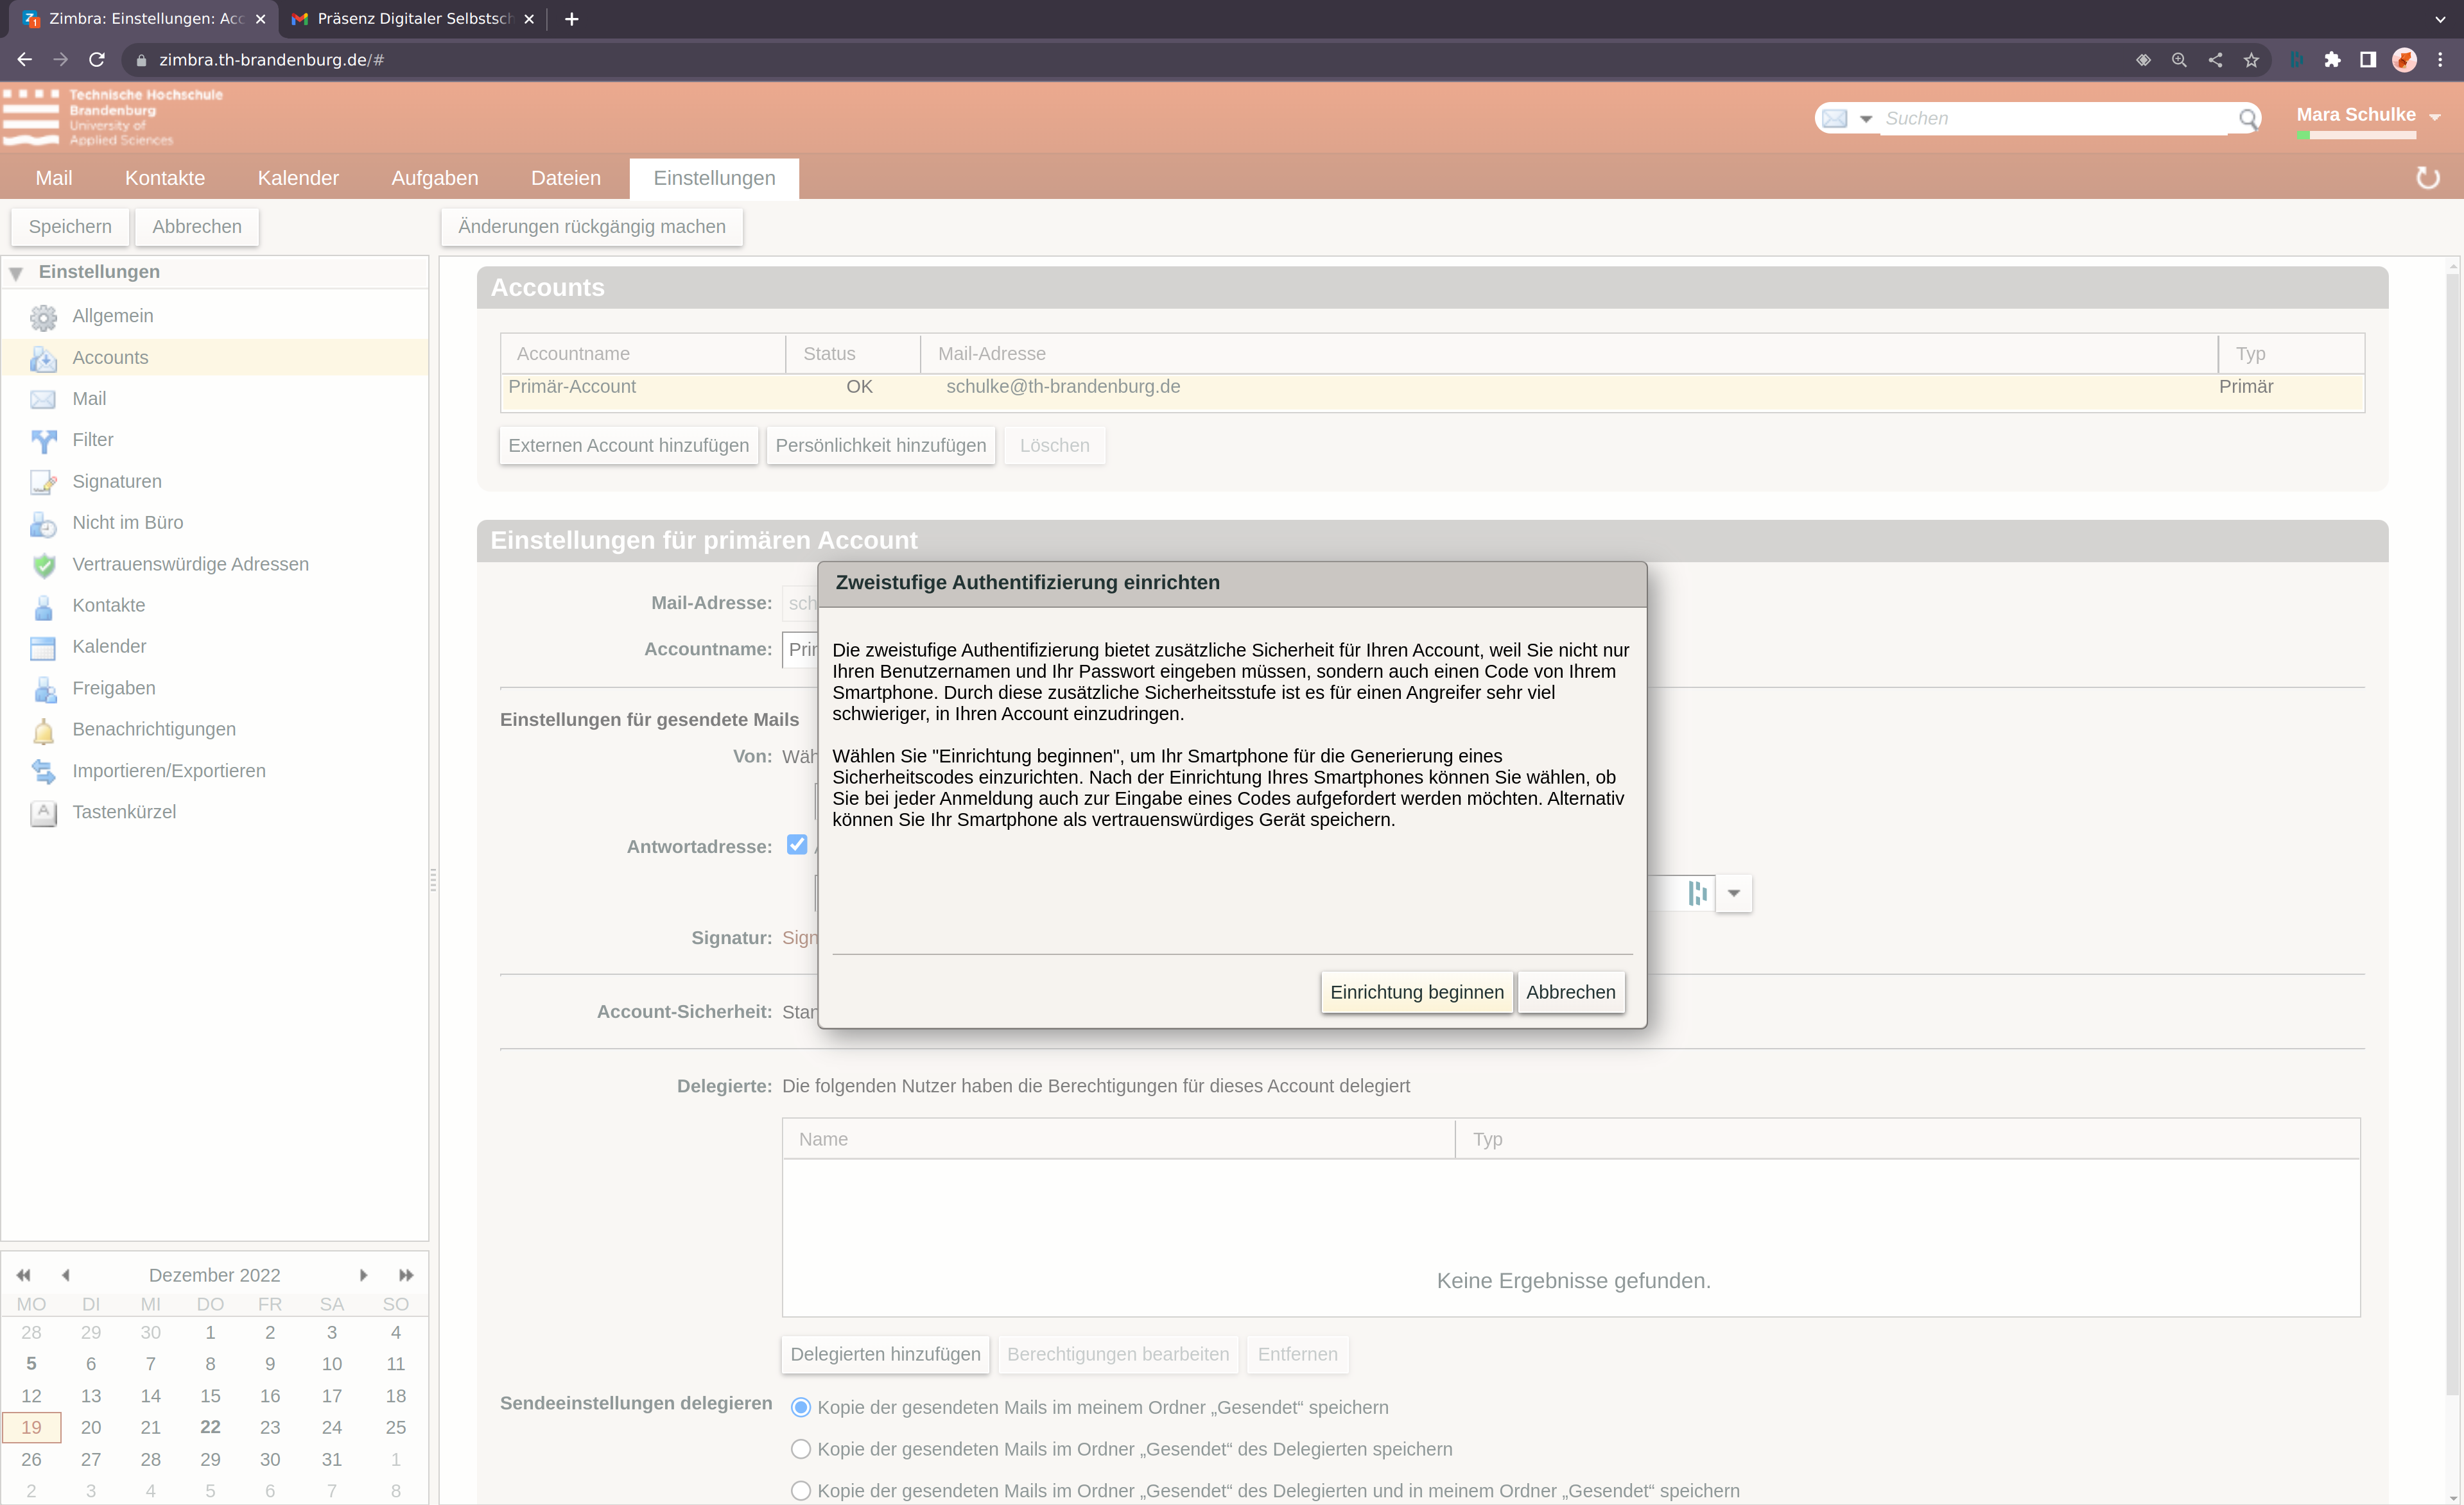
\includegraphics[width=0.75\textwidth]{./images/02-beginn.png}
	\centering
	\caption{Beginn der Einrichtung}
\end{figure}

Anschließend findet eine erneute Passwortabfrage statt, um die Identität des
Nutzers sicherzustellen, bevor eine eventuell zugriffsgefährendende Aktion (z.B.
bei Verlust des Smartphones und der Recovery-Codes) durchgeführt wird. (Abb. 3)

\begin{figure}[H]
	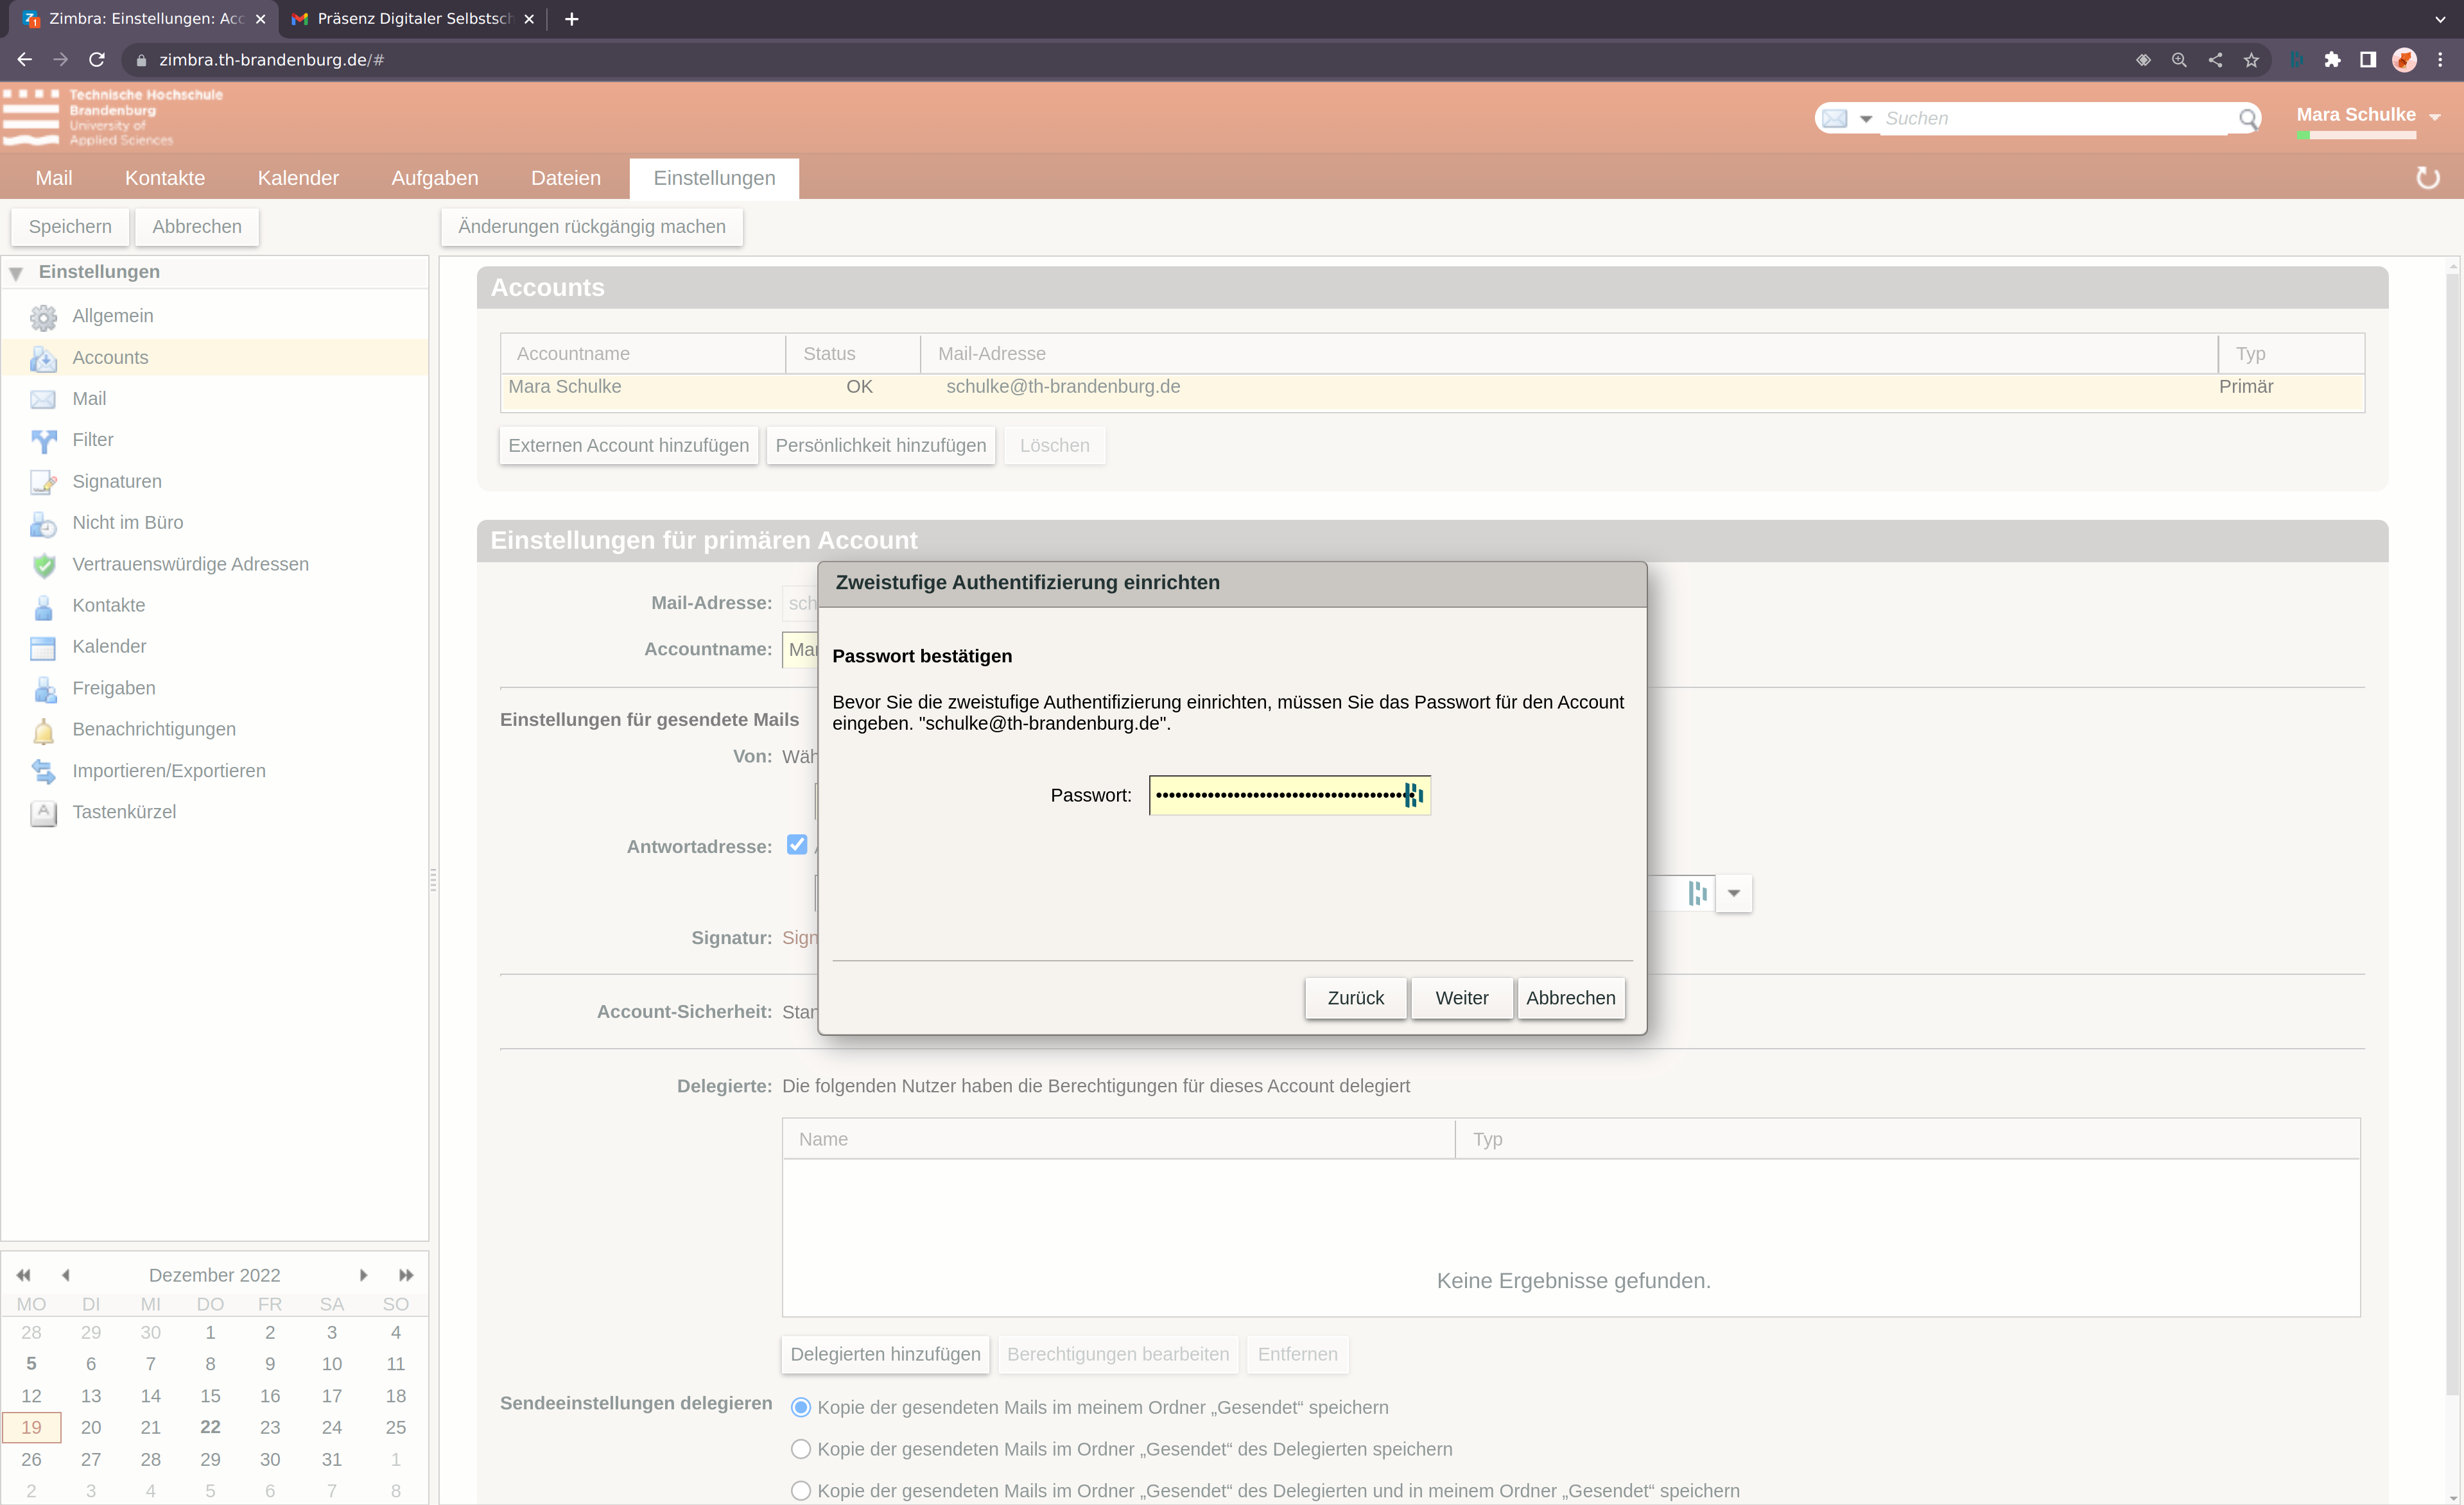
\includegraphics[width=0.75\textwidth]{./images/03-passwort.png}
	\centering
	\caption{Passwortabfrage}
\end{figure}

Nun wird das Geheimnis zur Generierung von One-Time-Passwords angezeigt. Dieses
muss nun in einen kompatiblen Authenticator eingegeben werden. (Abb. 4)

\begin{figure}[H]
	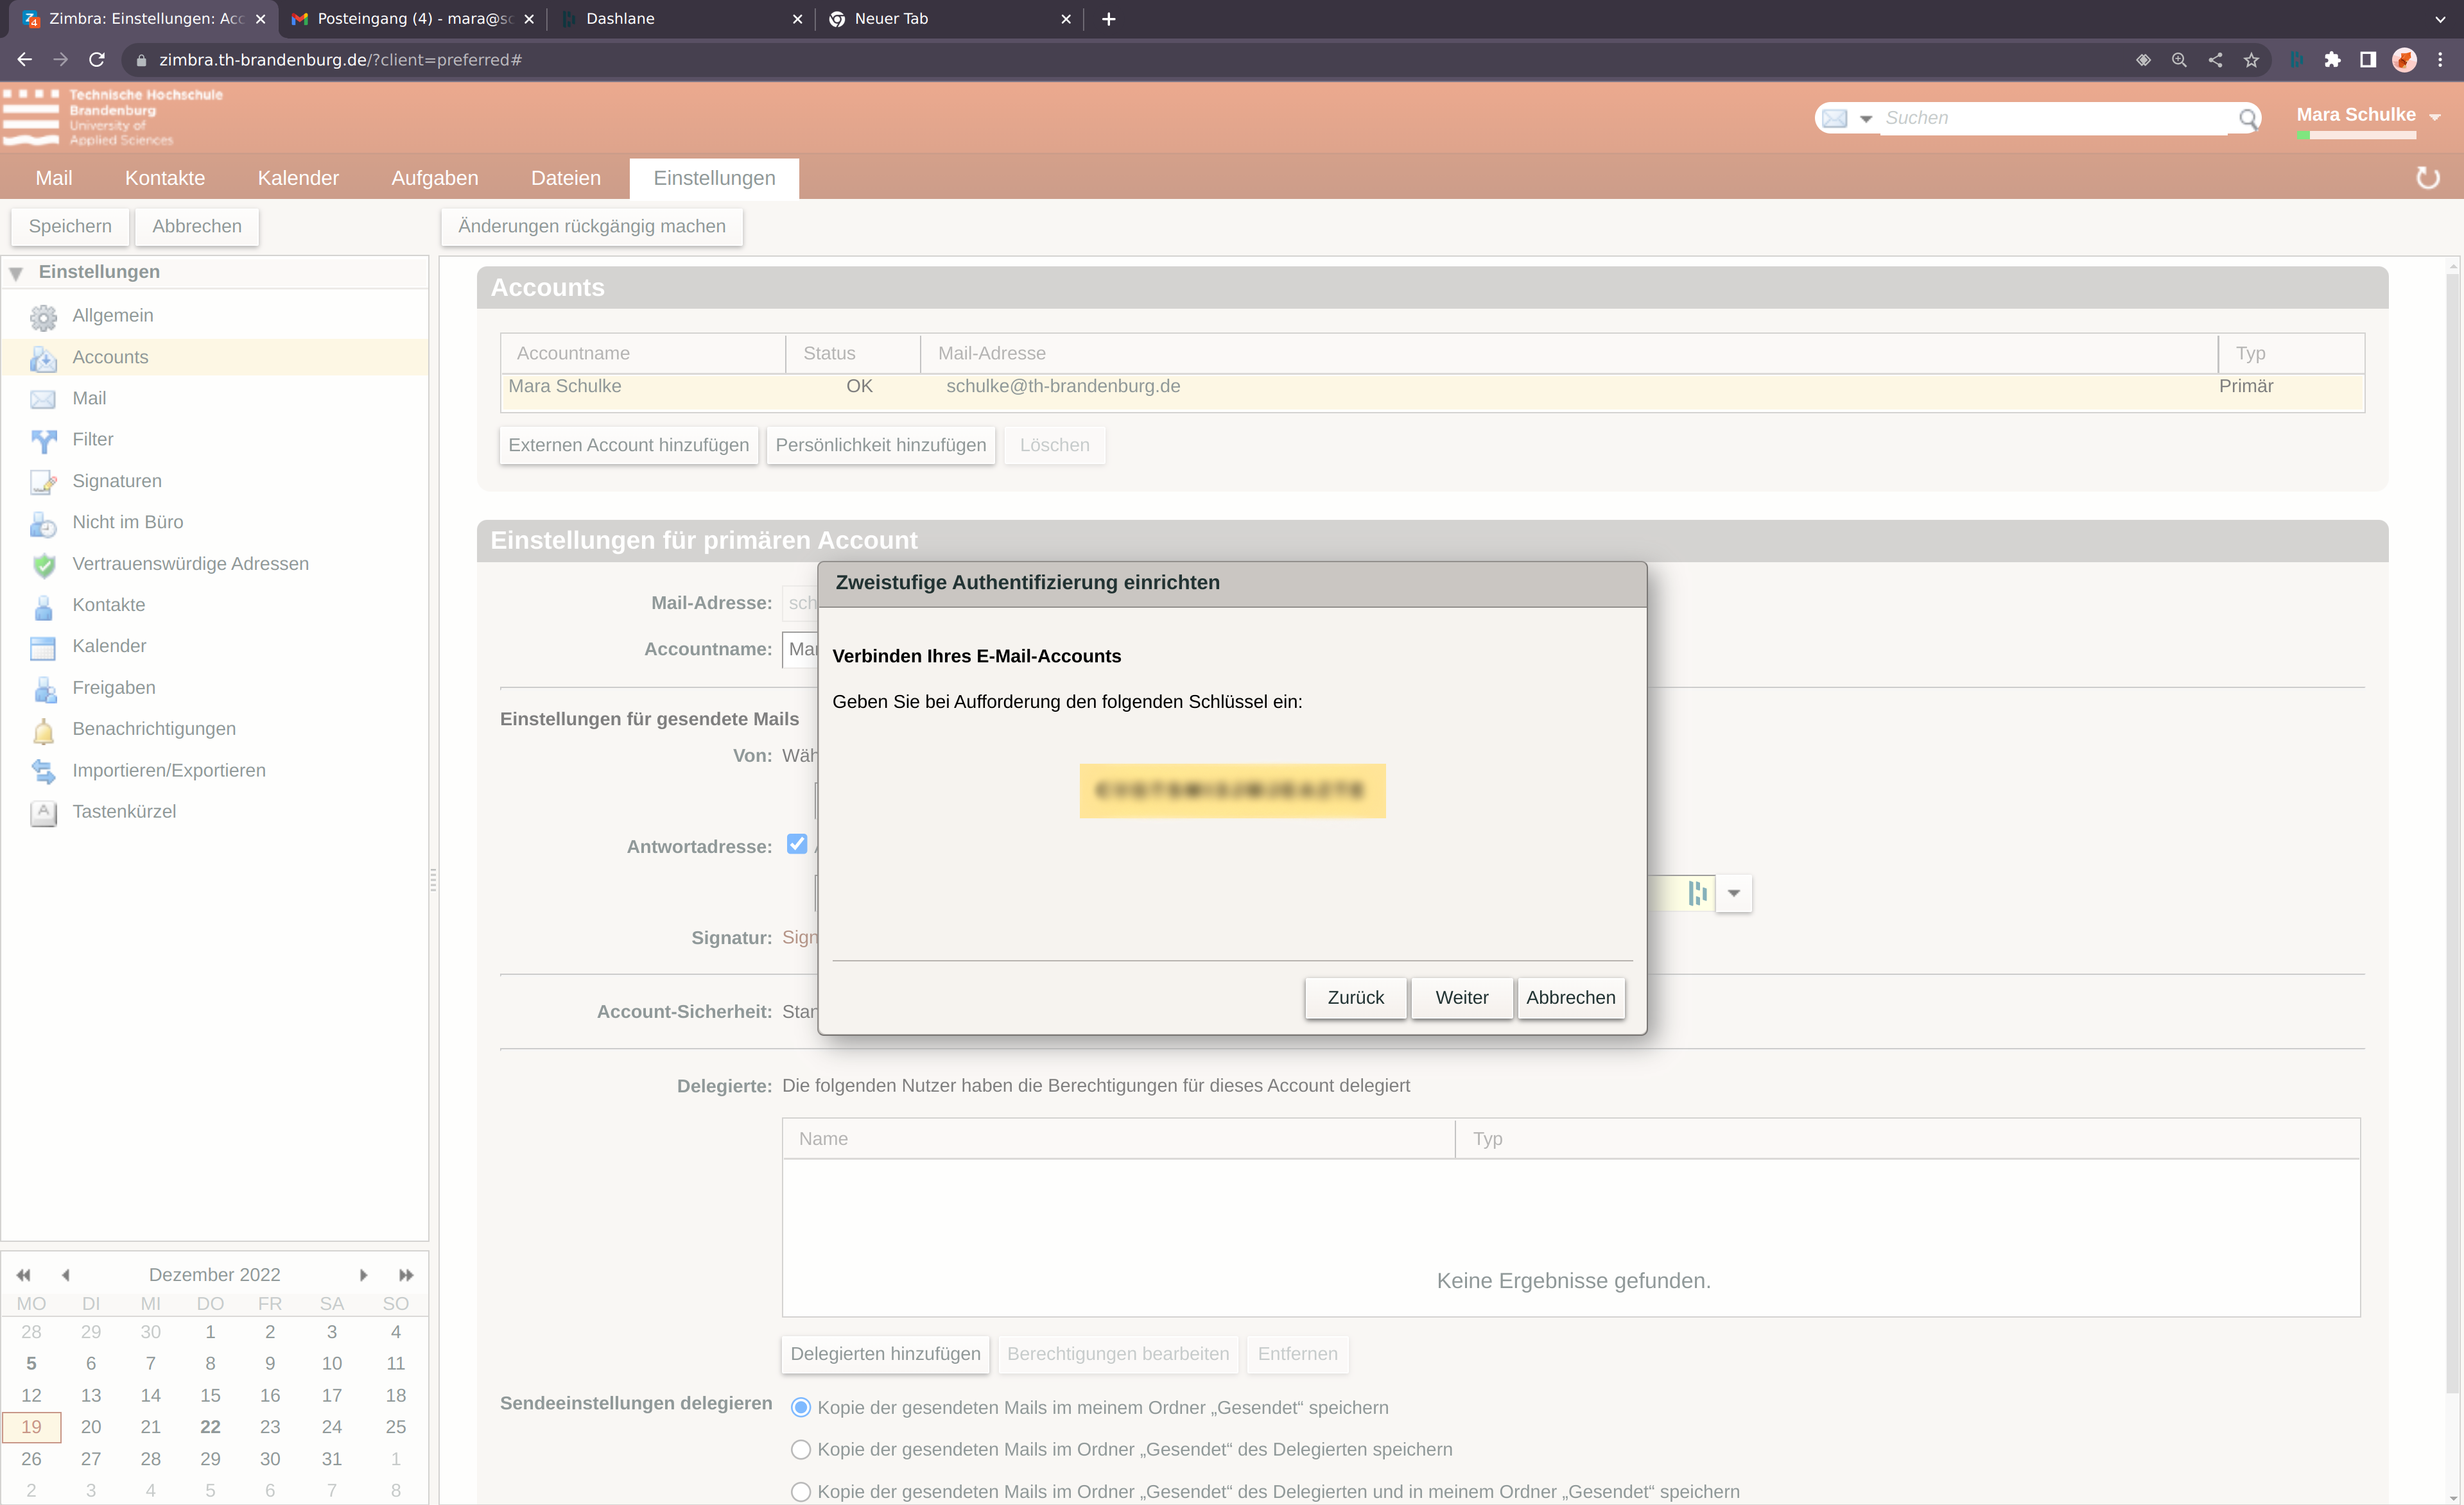
\includegraphics[width=0.75\textwidth]{./images/04-secret.png}
	\centering
	\caption{2-Faktor-Secret}
\end{figure}

Für meine persönliche Einrichtung habe ich mich für Dashlane entschieden, da
die One-Time-Passwords sehr übersichtlich direkt in dem Account-Eintrag
innerhalb des Passowrt-Managers auf dem Smartphone angezeigt werden. Es muss
nun das Geheimnis aus Abbildung 4 in den Authenticator eingetragen werden.
(Abb. 5)

\begin{figure}[H]
	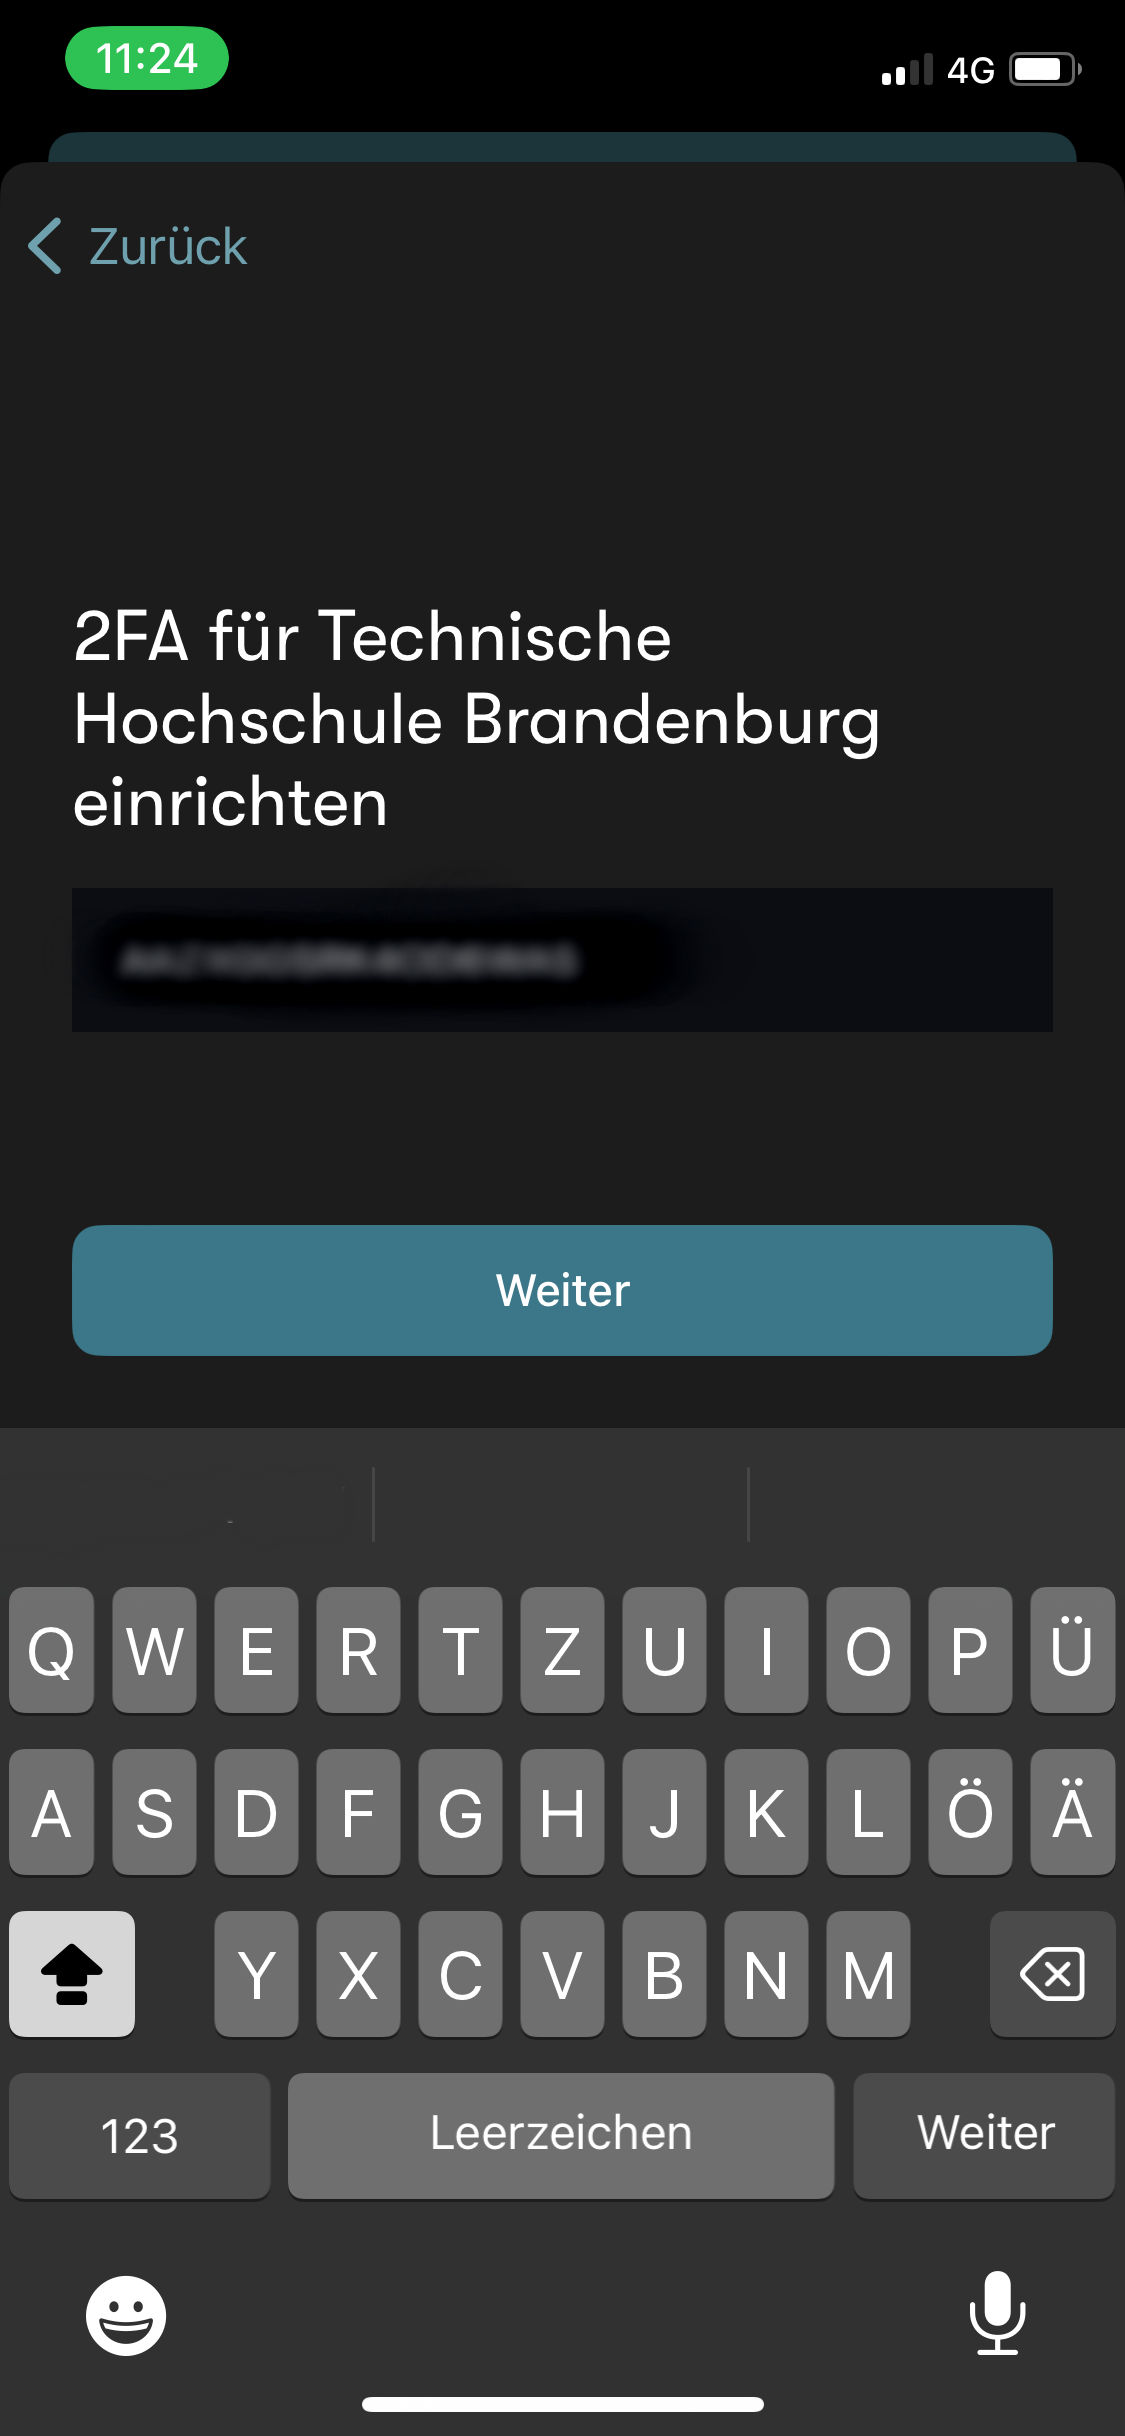
\includegraphics[height=0.25\textheight]{./images/05-eingabe-secret.png}
	\centering
	\caption{Eingabe des Secrets in Dashlane}
\end{figure}

Wenn die Eingabe erfolgreich war, bestätigt Dashlane dies und fängt sofort mit
der Generierung von 2-Faktor-Codes an. (Abb. 6\&7)

\begin{figure}[H]
	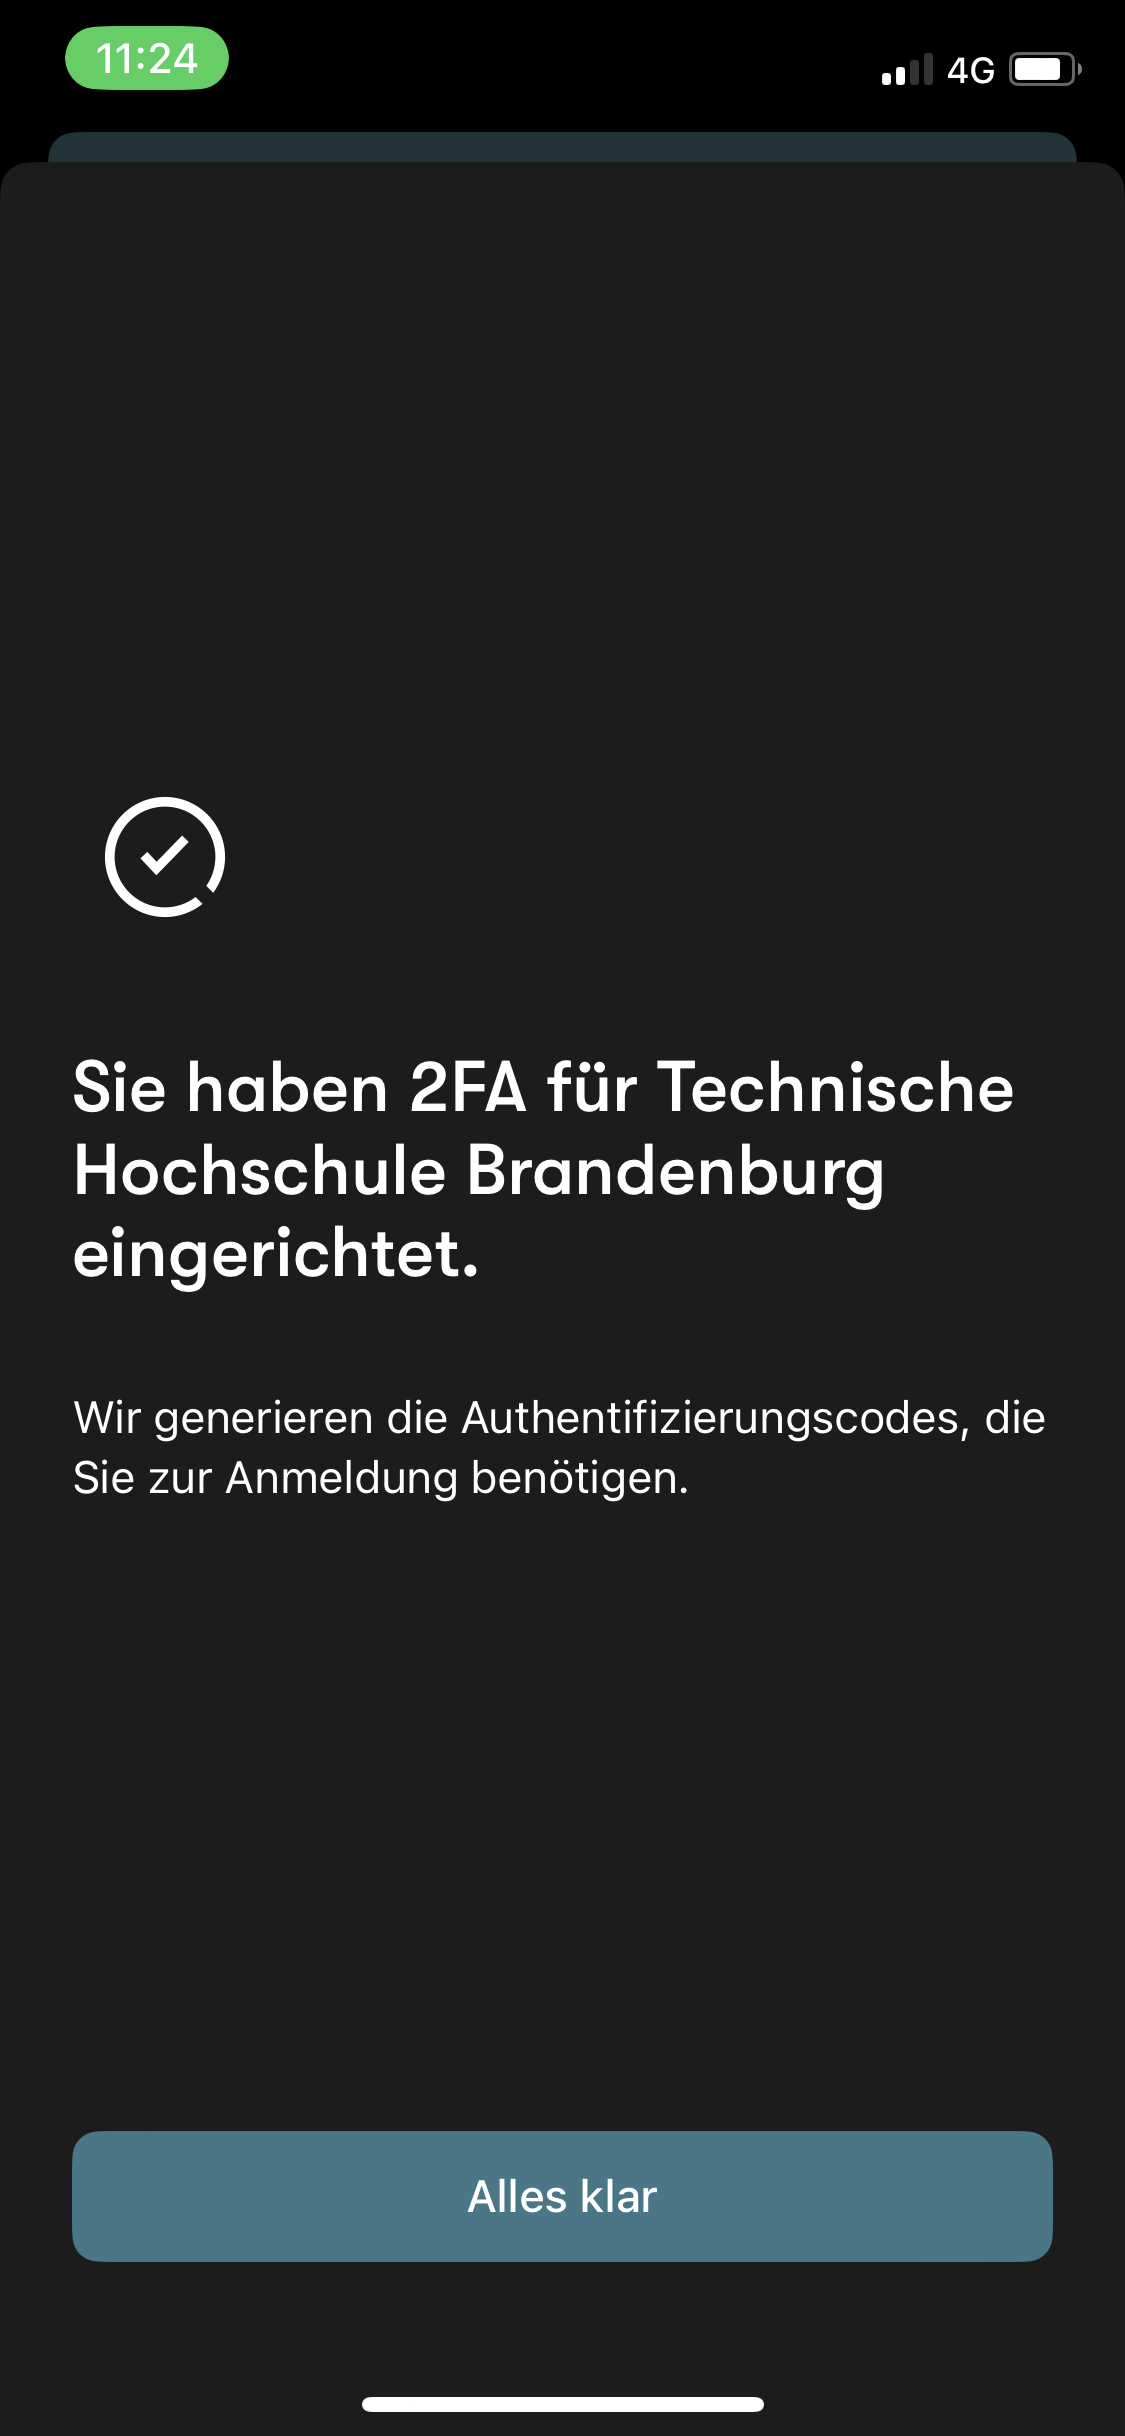
\includegraphics[height=0.25\textheight]{./images/06-erfolg.png}
	\centering
	\caption{Erfolg in Dashlane}
\end{figure}

\begin{figure}[H]
	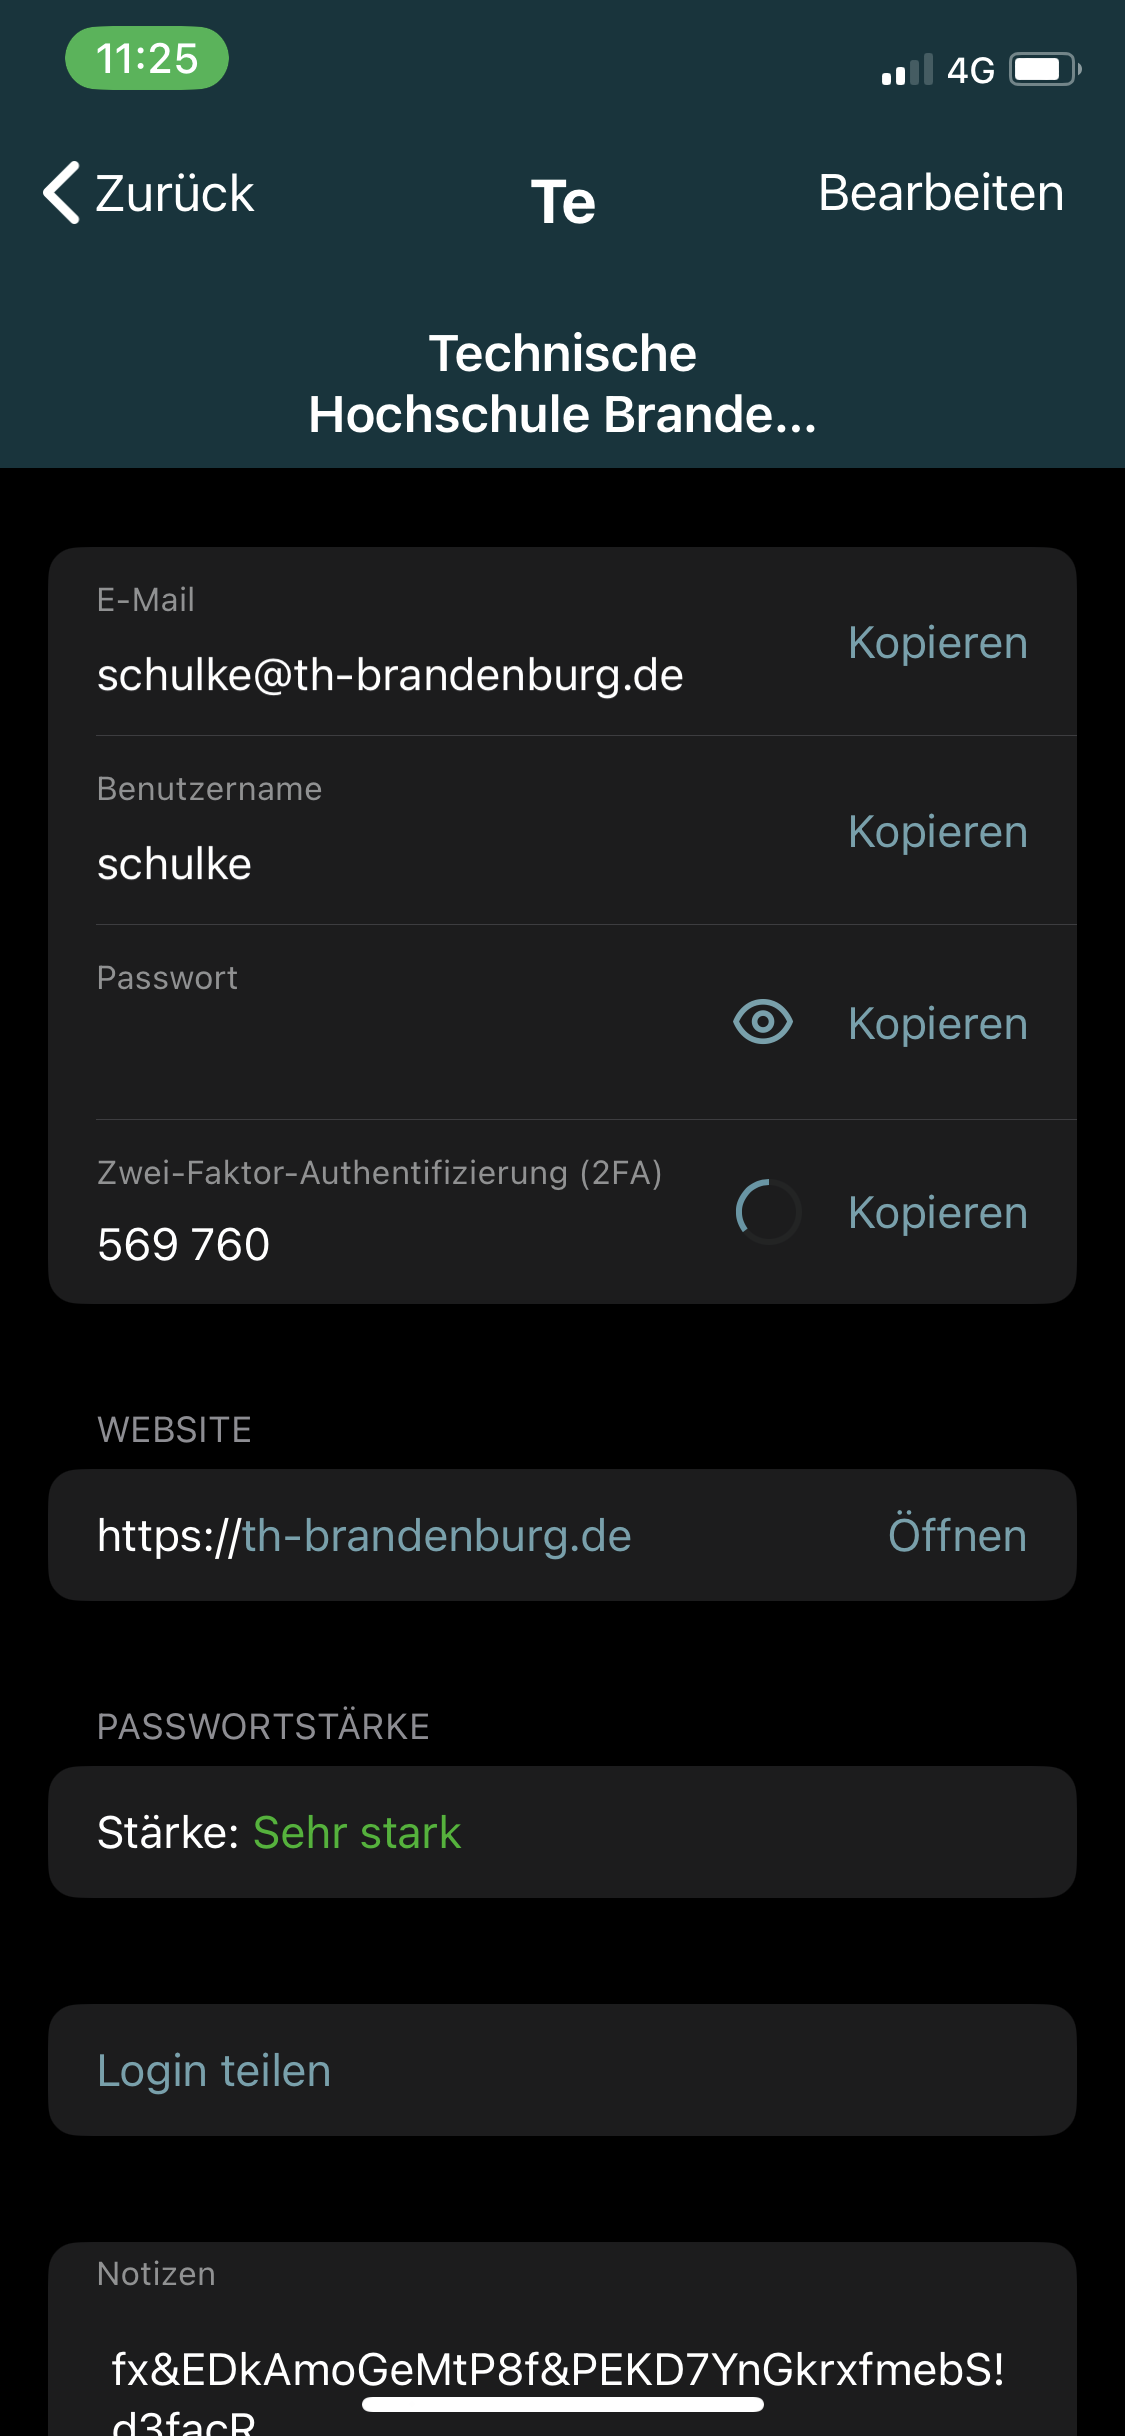
\includegraphics[height=0.25\textheight]{./images/07-code.png}
	\centering
	\caption{Generierter 2-Faktor-Code}
\end{figure}

Zimbra fordert nun den Nutzer auf, die erfolgreiche Einrichtung des
Authenticators zu bestätigen, in dem ein OTP angefordert wird. Die ist wichtig,
um zu verhindern, dass der Nutzer ein falsches Secret in seinen Authenticator
übertragen hat, das zwar auch OTPs generiert, die allerdings nicht für dieses
Secret gültig sind. (Abb. 8)

\begin{figure}[H]
	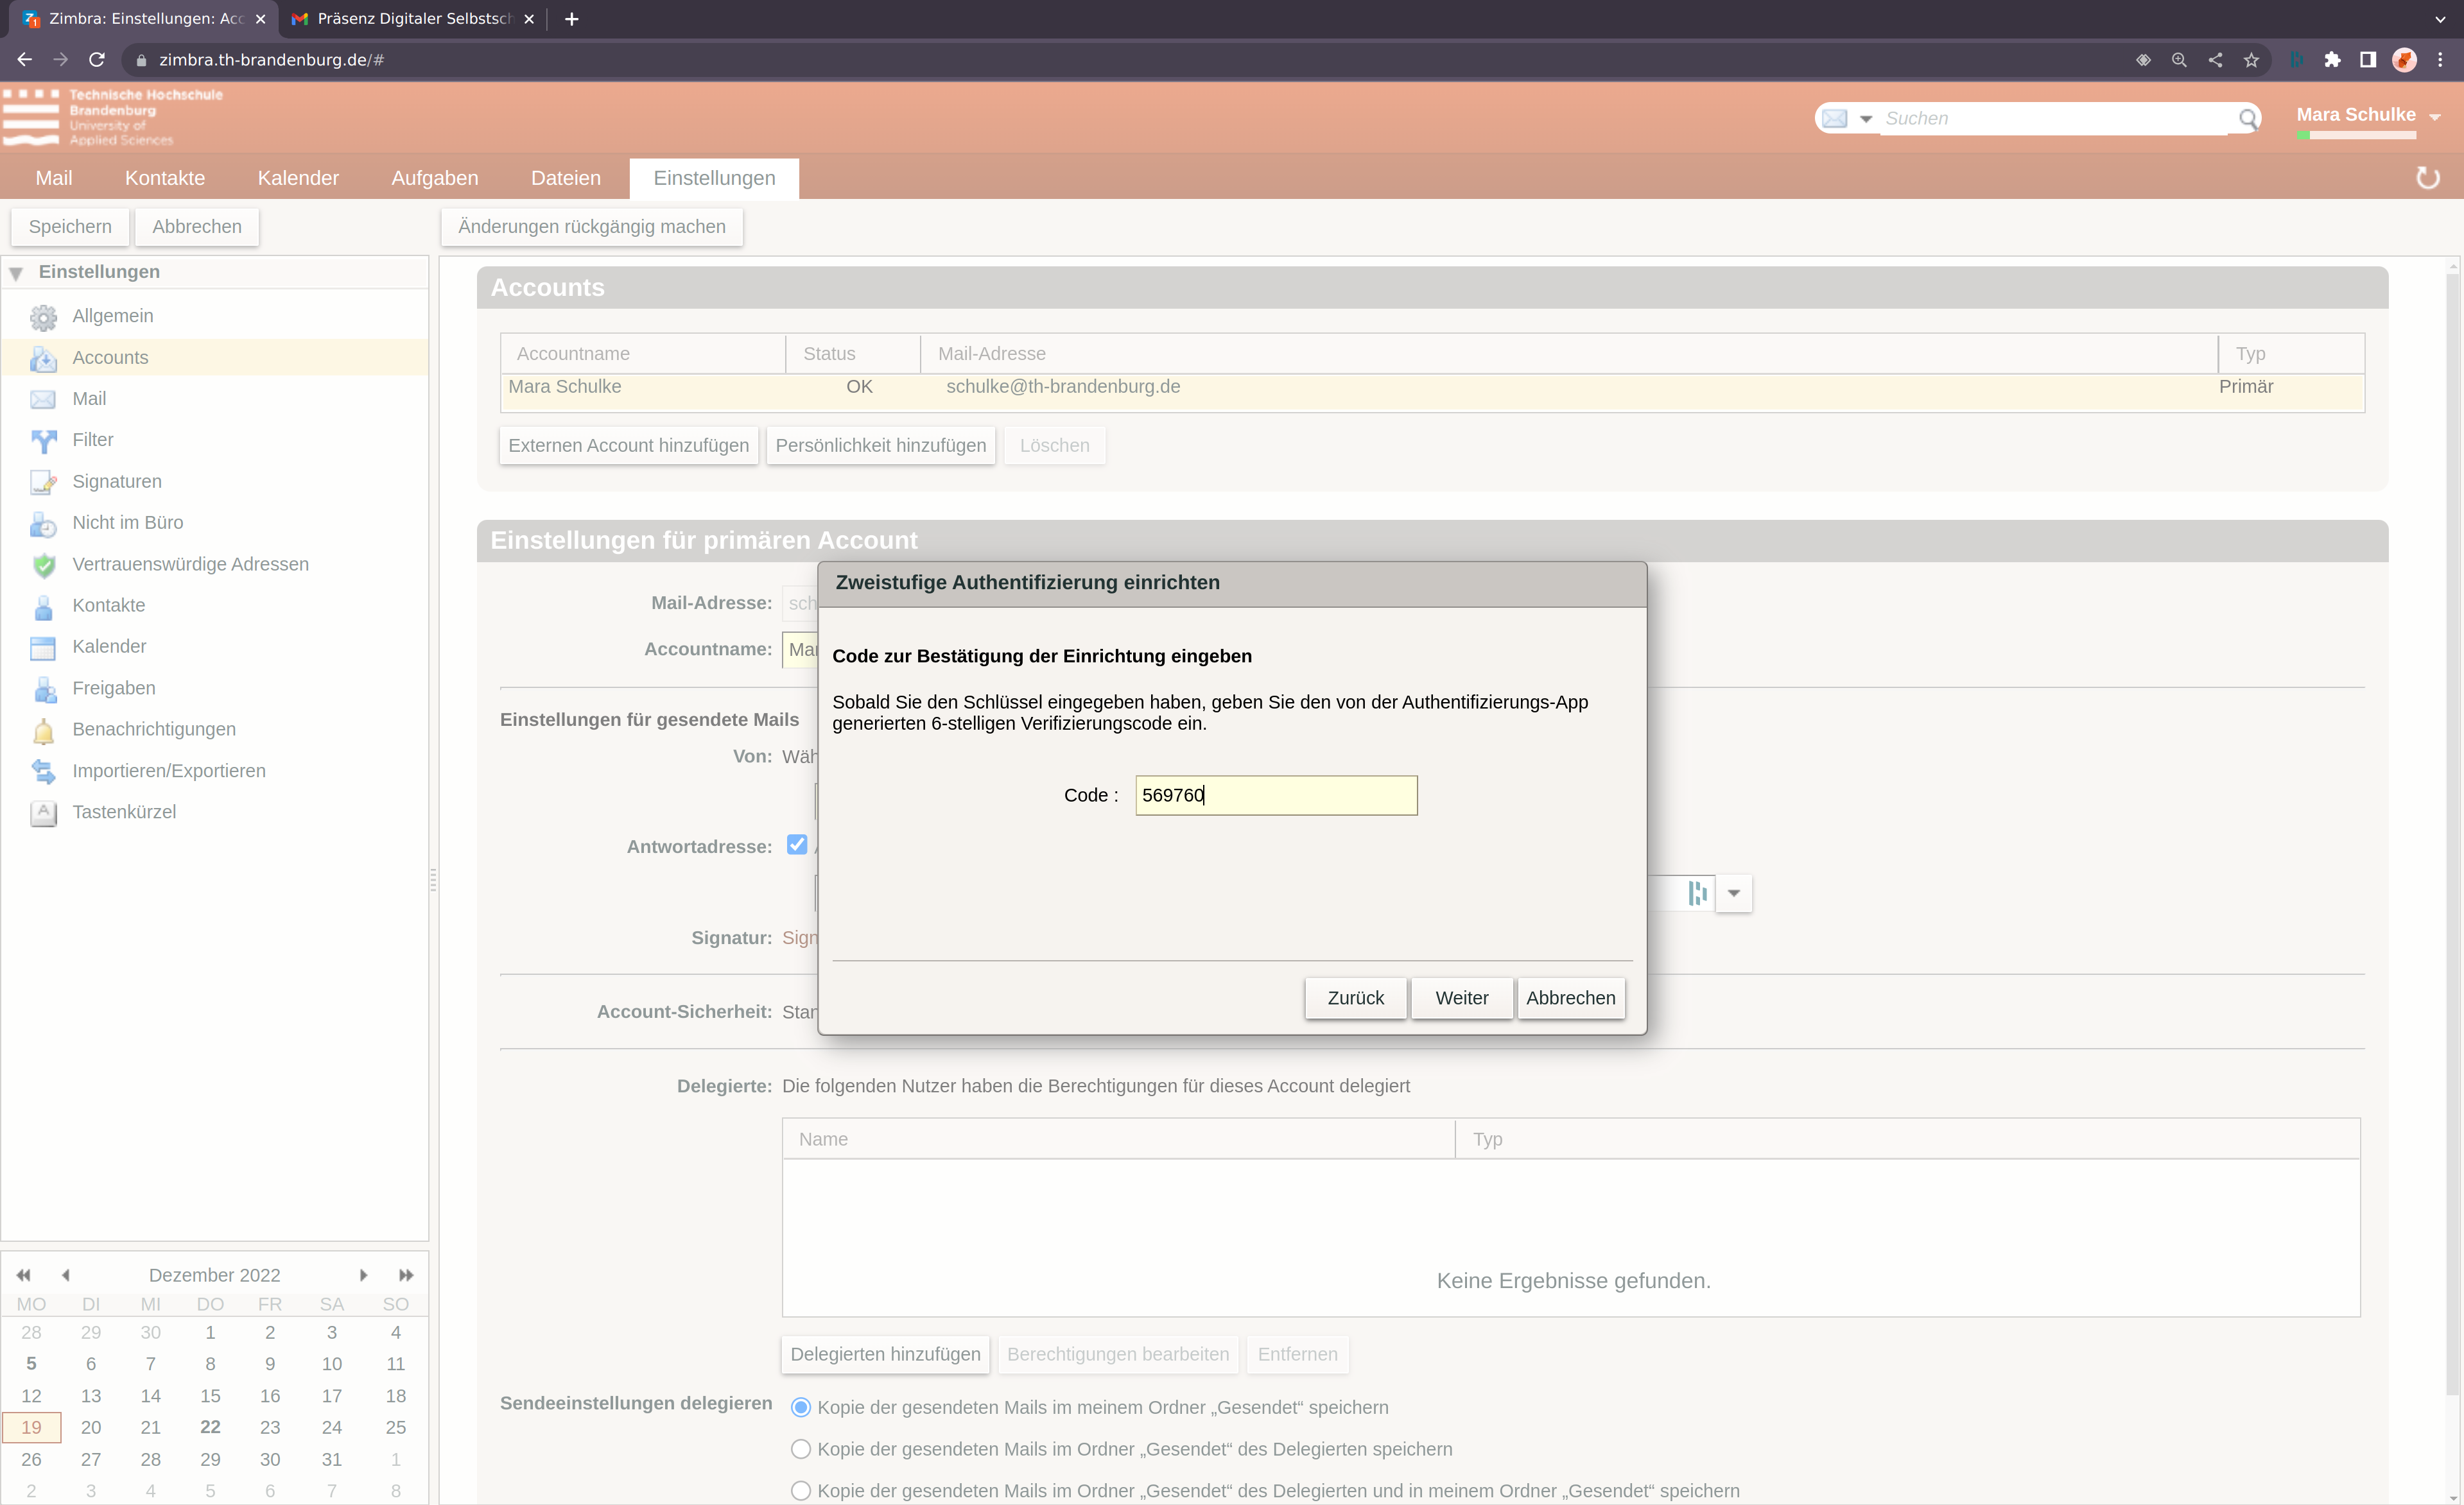
\includegraphics[width=0.75\textwidth]{./images/08-bestaetigung.png}
	\centering
	\caption{Bestätigung des Authenticators}
\end{figure}

Wenn das Geheimnis korrekt übertragen wurde und der Authenticator funktioniert
und gültige One-Time-Passwords ausgibt, zeigt Zimbra nun eine Bestätigung der
erfolgreichen Einrichtung an. (Abb. 9)

\begin{figure}[H]
	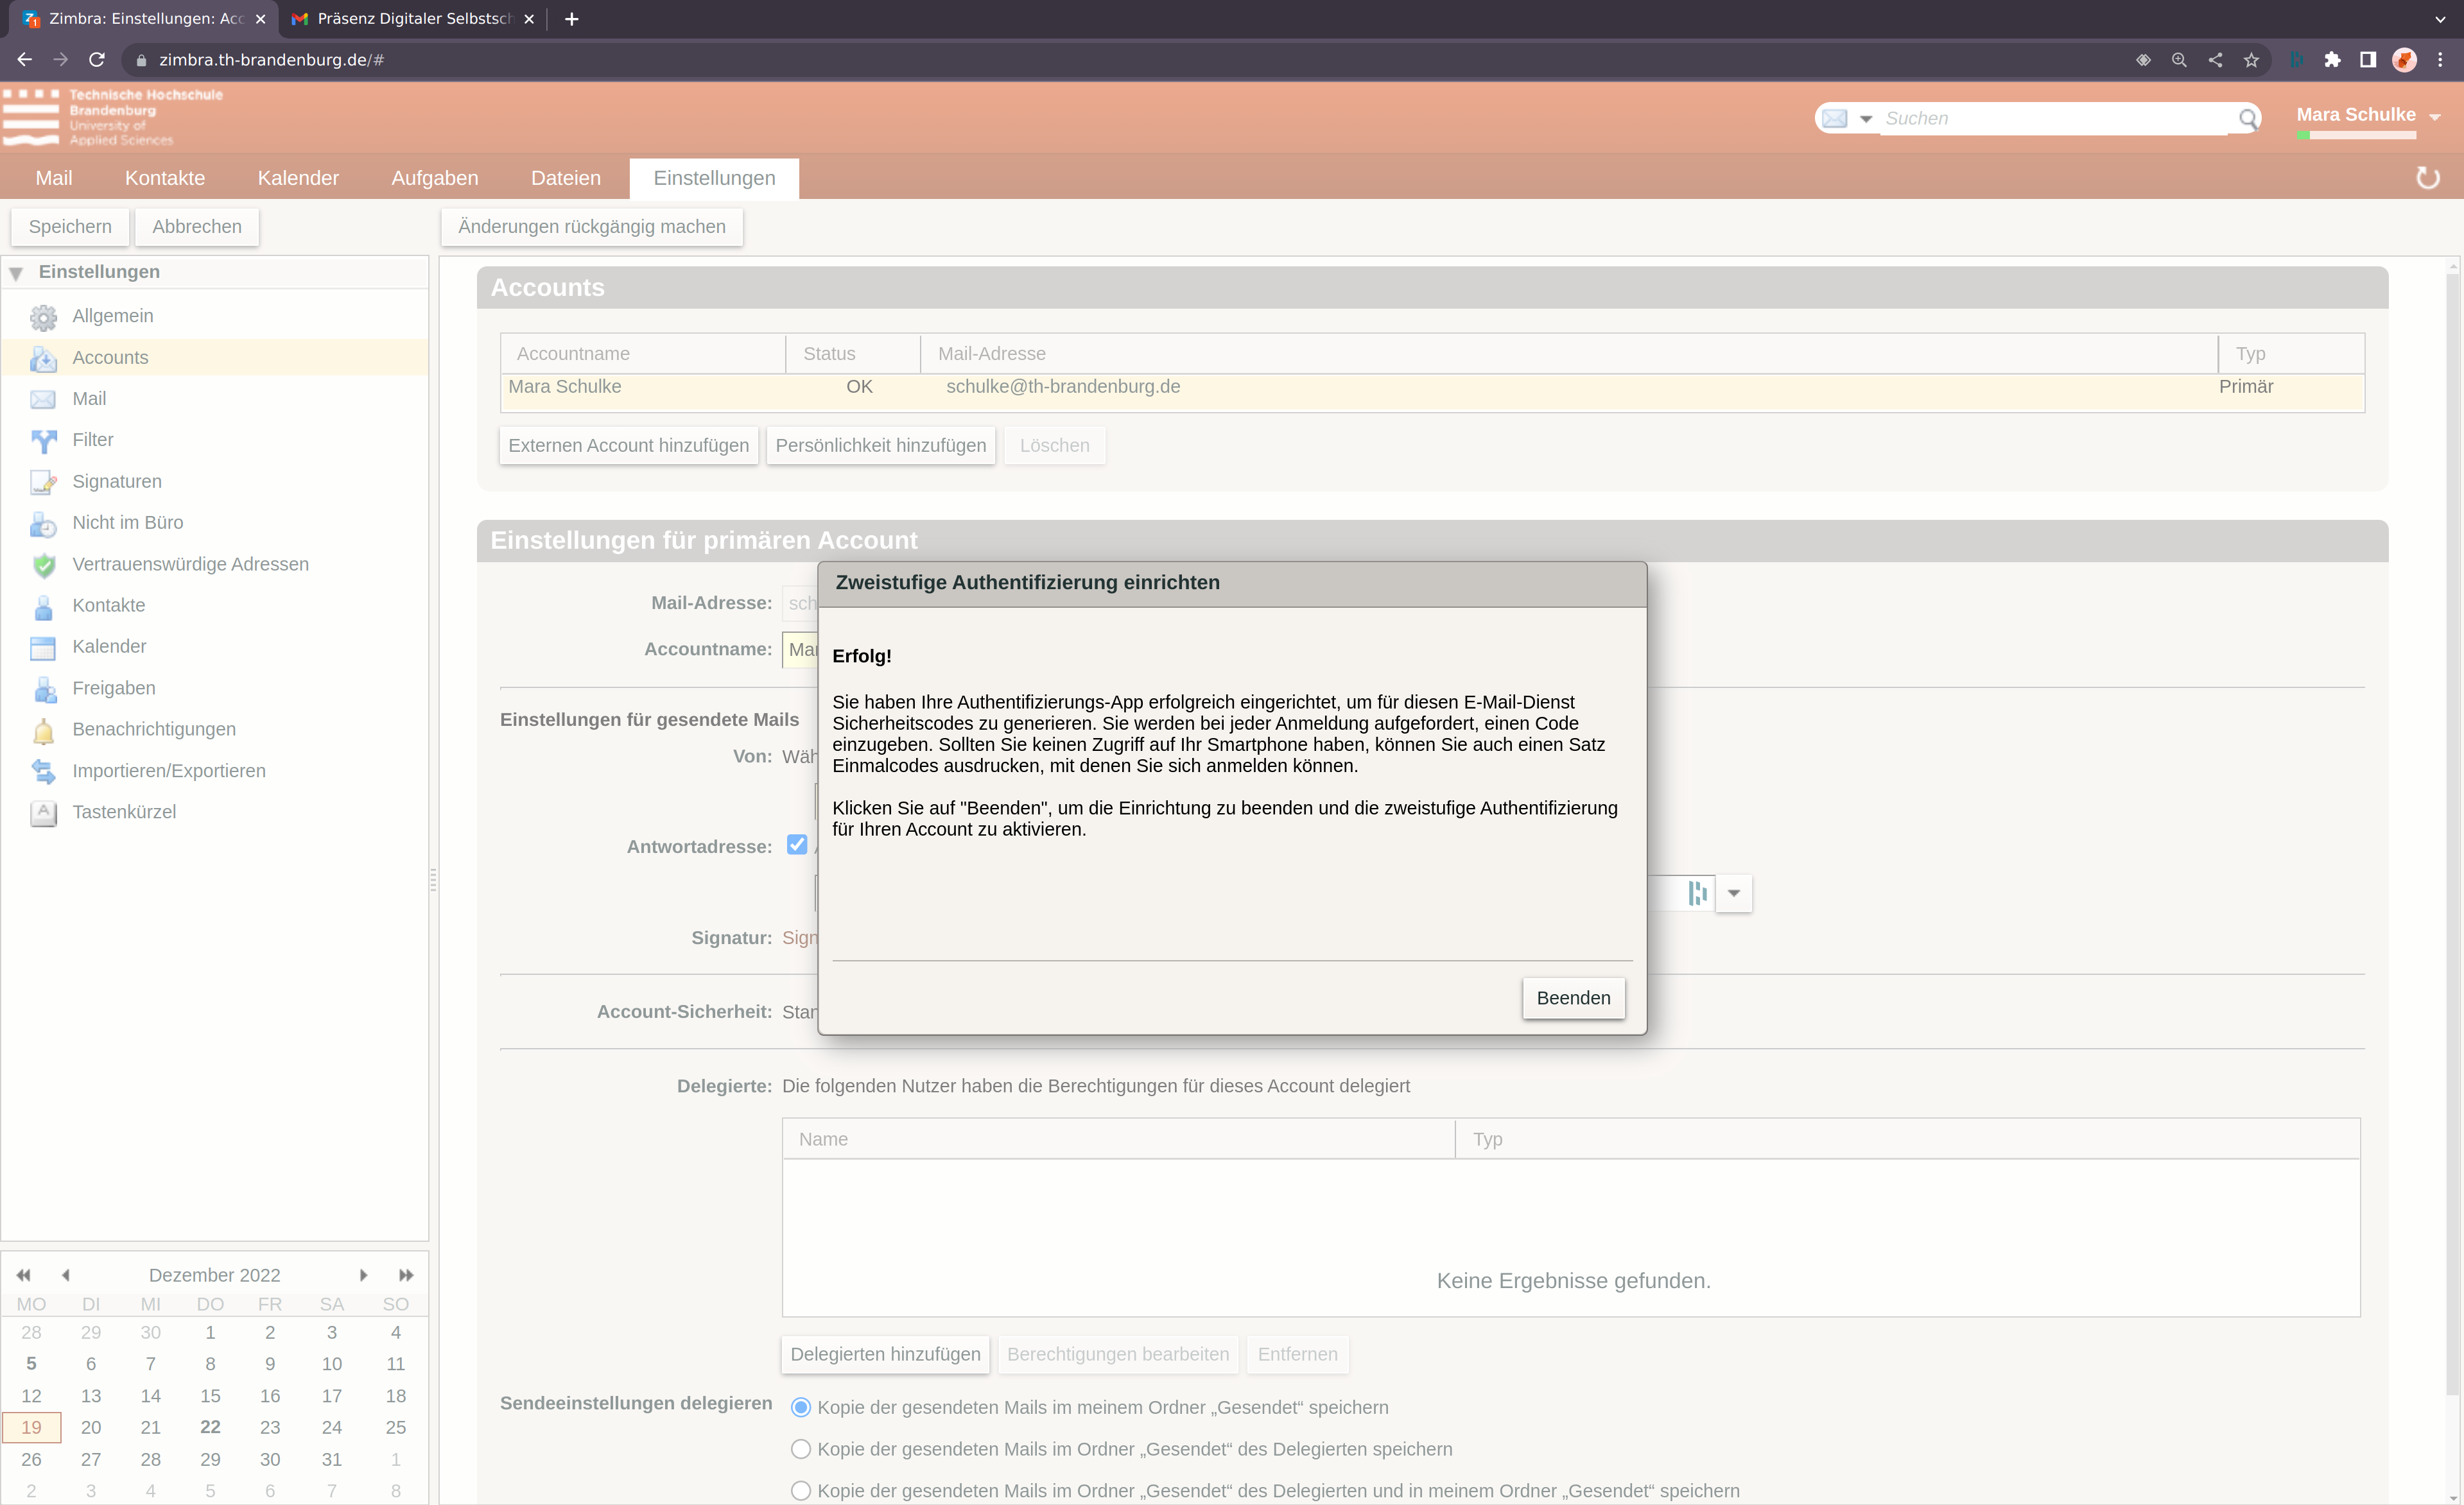
\includegraphics[width=0.75\textwidth]{./images/09-erfolg-zimbra.png}
	\centering
	\caption{Erfolgreiche Einrichtung}
\end{figure}

Bevor nun mit der alltäglichen Nutzung fortgefahren wird, ist es wichtig, die
Recovery-Codes an einem sicheren Ort ausserhalb des für 2FA verwendenten Gerätes
abzulegen. Sollten die Recovery-Codes auf dem gleichen Gerät abgelegt werden,
sind sie im Falle eines Verlusts nicht greifbar und somit nutzlos zur
Wiederherstellung. (Abb. 10) In meinem Beispiel habe ich diese in die Notizen des
THB-Eintrags innerhalb meines Passwort-Managers gespeichert, da ich diese auch
bei einem eventuellen Verlust meines Smartphones erreichen könnte.

\begin{figure}[H]
	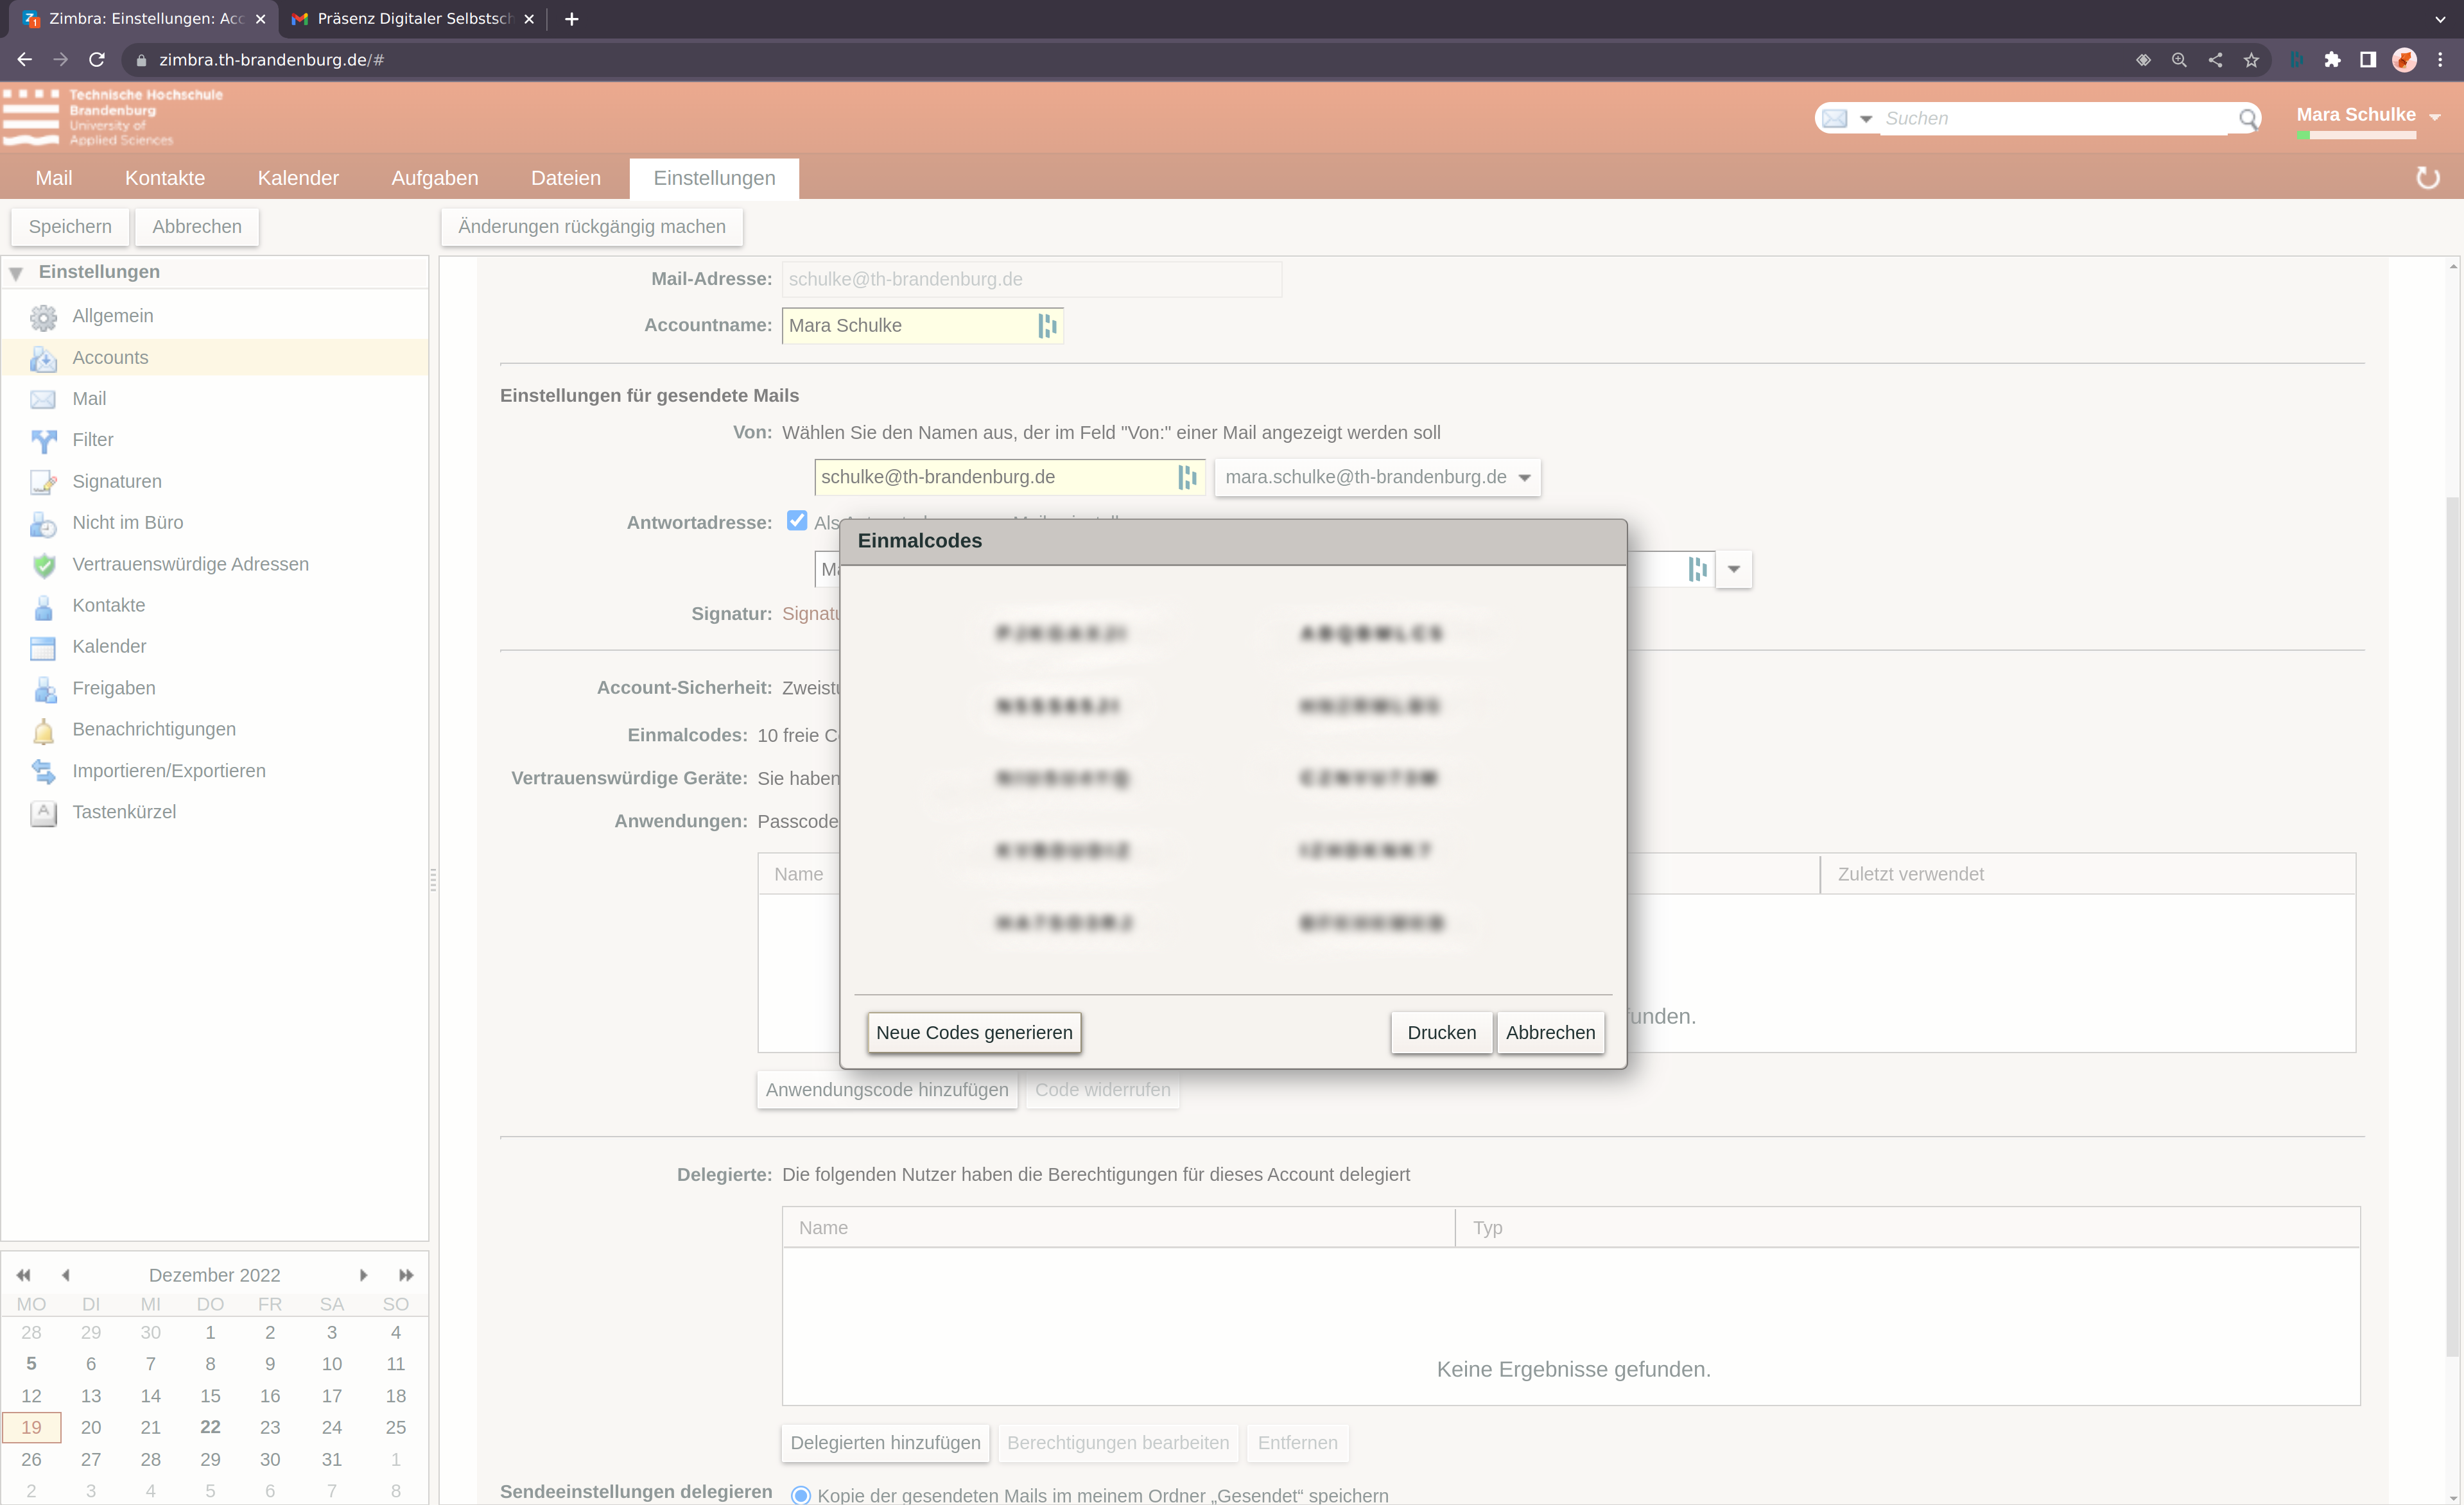
\includegraphics[width=0.75\textwidth]{./images/10-recovery-codes.png}
	\centering
	\caption{Ausgabe der Recovery-Codes}
\end{figure}

Nach der erfolgreichen Einrichtung kann der zweite Faktor nun erneut getestet
werden, indem sich der Nutzer einmal ausloggt und erneut anmeldet. Nun sollte
Zimbra nach erfolgreicher Eingabe der Login-Daten ein One-Time-Password
abfragen, welches aus dem Authenticator übertragen werden kann. (Abb. 11)

\begin{figure}[H]
	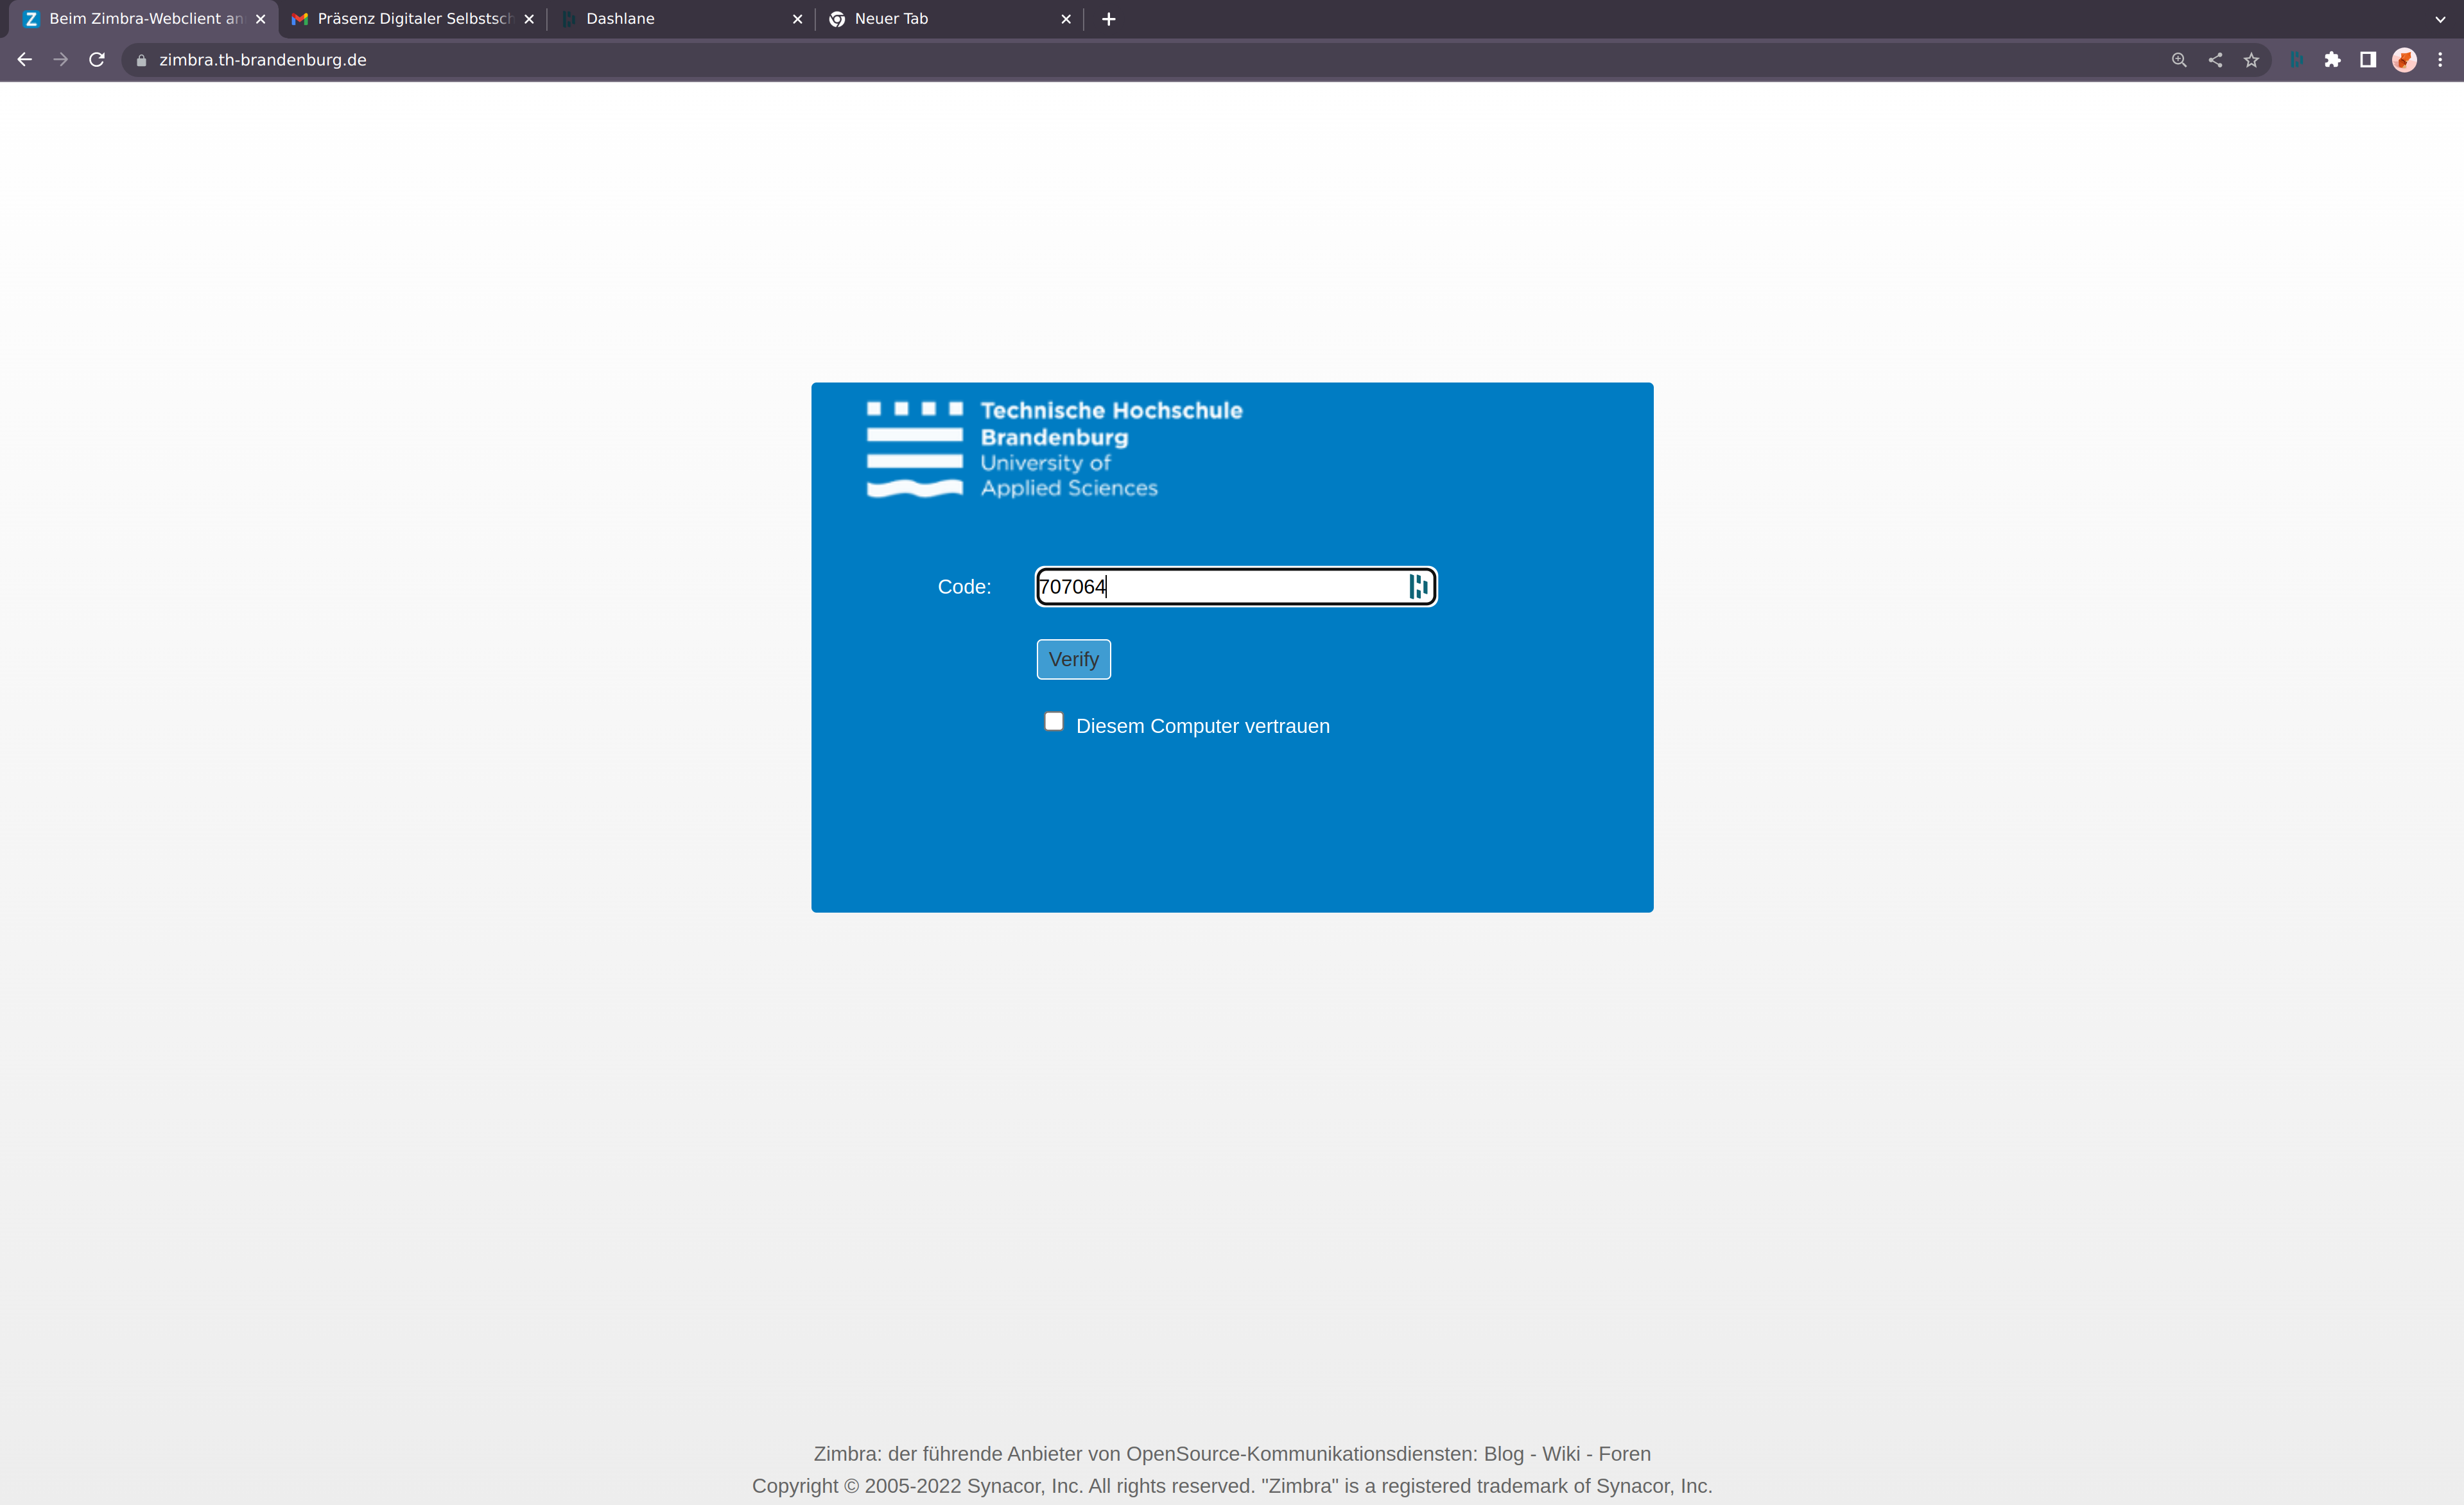
\includegraphics[width=0.75\textwidth]{./images/11-login-2fa.png}
	\centering
	\caption{Login bei Zimbra nach Einrichtung}
\end{figure}

\section{Erfahrungsbericht}

Die Einrichtung einer 2-Faktor-Authentifizierung ist im Allgemeinen ein
vergleichsweise kleiner Aufwand für die Sicherheitsgarantien, die diese bietet.
Durch die gängigen Anwendungen für Mobilgeräte (beispielsweise Google
Authenticator, Authy etc.) gestaltet sich die Einrichtung im Rahmen eines
Regestrierungsprozesses und die Anwendung im Alltag in der Regel
nutzerfreundlich (zum Beispiel durch die Verwendung von QR-Codes als
Einrichtungshilfe).

Im Gegensatz zur reinen wissensbasierten Authentifizierungsmethode
(üblicherweise Passwörter) birgt die 2-Faktor-Authentifizierung (insbesondere
TOTP) das Risiko des Verlustes des Endgerätes. Der Nutzer kann somit trotz
berechtigter Absicht (Zugriff auf den eigenen Account) nicht beweisen, dass es
sich um die richtige Person handelt. Als Lösung werden oftmals Recovery-Codes
eingesetzt, die der Nutzer an einem Ort außerhalb des für die
2-Faktor-Authentifizierung verwendenten Gerätes speichern. Diese bieten jeweils
einmaligen Zugriff auf den Account, um beispielsweise ein neues Gerät bei
Verlust des alten zu konfigurieren. Die sichere verwarung von Recovery-Codes
ist zwingend erforderlich, um die Sicherheitsgarantien der
2-Faktor-Authentifizierung zu bewahren, da beispielsweise bei einer
ungeschützten Aufbewahrung auf einem Schreibtisch im Großraumbüro die
Möglichkeit eines Angriffes besteht. Dieser ist zwar immer noch im Vergleich
zur reinen wissensbasierten Authentifizierung erschwert, da ein Angreifer in
dem gerade genannten Beispiel physischen Zugriff auf den Schreibtisch
erlangen müsste, aber dennoch deutlich vereinfacht im Vergleich zu einem
Brute-Force-Angriff auf 2-Faktor-Geschützte Accounts.

Im Falle von Zimbra ist die Einrichtung einerseits verständlich und
nutzerfreundlich gestaltet, sobald der Einreichtungsassistent geöffnet ist,
allerdings wäre die Verwendung eines QR-Codes aus Nutzersicht empfehlenswert,
da dies das mühsame Abtippen des geheimen TOTP-Schlüssels in die
Authenticator-App abkürzen würde. Sobald die Einrichtung abgeschlossen ist,
läuft alles in einer zu anderen Anwendungen vergleichbaren Weise ab (Zeitpunkt der
TOTP-Aufforderung, Recovery-Codes, Entfernen vom Authenticator etc.). Somit
kann festgestellt werden, dass die Einrichtung der 2-Faktor-Authentifizierung
bei richtiger Anwendung eine deutlich höhere Sicherheit bietet und bei
geringer Beeinträchtigung des Nutzererlebnisses verpflichtend eingeführt werden
sollte.

\end{document}
